% !TEX root = main.tex
\chapter{Simulation Results}\label{cha:result}
This section describes the simulation results considering performance, robustness and stability with respect to the different control approaches. All approaches will first be benchmarked with the present control approach and presented individually in the following subsections. Comparison tables outlining the performance and the robustness of each controller will be presented in the end of this chapter.

\section{Benchmarking Tests}
For the comparison with the present control approach, all evaluated controllers were discretized with a sampling frequency of 2kHz. The normalized system in \eqref{eq:tf} was used to model the rotational stage linear dynamics. The nonlinear dynamics, creep and hysteresis, were neglected in the simulations, assuming perfect inverse hysteresis cancellation and a sufficient closed loop to compensate for the creep effect. All simulations were performed in Matlab and Simulink. The \abbrMRACPE and the \abbrIRC has been evaluated with respect to robustness to model errors, disturbance rejection, closed loop bandwidth and response to step and periodical input, all listed below.

\begin{itemize}
\item {\bf Step, ramp and periodical tracking} - A step and a periodical input is applied to the input to benchmark the tracking capability of the controller.
\item {\bf Disturbance rejection} - Impulses are added to the input and output signal of the system to benchmark how sensitive the system is to system disturbances.
\item {\bf Robustness to model errors} - The robustness to model errors is characterized by changing the dynamical model but keeping the model in the controller constant, either during runtime or instantaneously.
\end{itemize}

The \abbrIMP, the \abbrFDC and the \abbrRFDC have been evaluated with respect to cancellation effectiveness and robustness to model errors, as listed below.

\begin{itemize}
\item {\bf Cancellation performance} -  Sinusoidal signals or acquired noise from the lab is added as disturbance to test the cancellation performance.
\item {\bf Robustness to model errors} - The robustness to model errors is characterized by changing the dynamical model of the system but keeping the model in the controller constant.
\end{itemize}

The prospective challenges, described in \ref{sec:prospectiveChallanges} shall be kept in mind while reading the results. Since the required ramp rates are relatively low, the disturbance rejection and the robustness to model errors are more of interest when evaluating each method.

\section{Linear Dynamics Characterization}
The linear dynamics of the rotational stage changes due to the a number of physical properties of the system, such as the current yaw-position, the linear axis position and speed and if the system is in contact with the end-switches. This phenomenas were characterized in a number of tests and summarized below. Figure~\ref{fig:different_angles} shows a comparison of the identified model when the linear axis is in its outer position and the rotational head has rotated -10 mrad (0V), 0 mrad (3.25V) and 10 mrad (6.5V). It shows that the system changes its first resonance peak as much as 15.3 Hz.

\begin{figure}[h!]
  \centering %crop: left bottom right top
  \subfloat[][\label{fig:different_angles}Different rotational head positions]{
  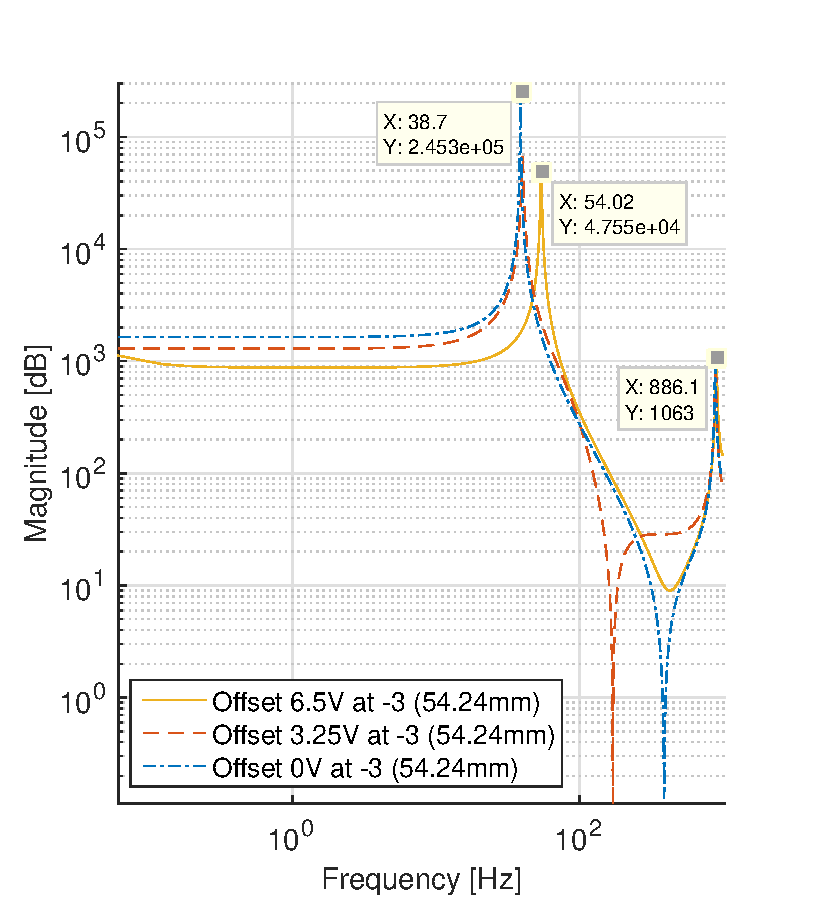
\includegraphics[width=0.46\textwidth, trim=0cm 0cm 0.8cm 1cm, clip=true]{fig/matlab/modelcomparison_diffvolt2.eps}}
  \qquad
  \subfloat[][\label{fig:different_lin_pos}Different linear axis positions]{
  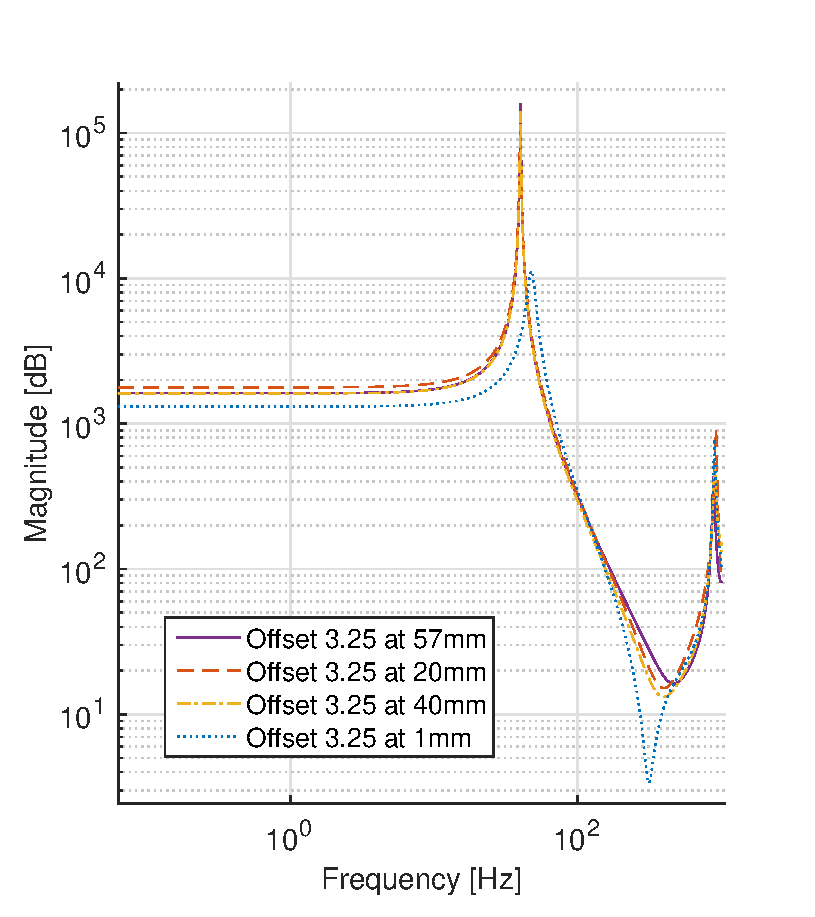
\includegraphics[width=0.46\textwidth, trim=0cm 0cm 0.8cm 1cm, clip=true]{fig/matlab/modelcomparison2.eps}}
  \caption{\label{fig:different_lin_angle} Identified models with different rotational positions (a) and linear axis positions (b).}
\end{figure}

Figure~\ref{fig:different_lin_pos} shows a comparison of the identified model when the rotational head is in 0 mrad (3.25V) and the linear axis position is in 1, 20, 40 and 57mm. The identified system are almost the same for the first 3 positions, but it changes drastically when the linear axis touches the outer switches in 57mm.

Since the rotational stage controller needs to maintain the required tracking error even when the linear axis is moving, the disturbance during linear operation must be considered. Figure~\ref{fig:dist_diff_speed} shows the open loop response when the linear axis is moving. This figure shows how the operating speed of the stepping motor influences the spectrum of the angle with its different harmonics.

\begin{figure}[h!]
  \centering %crop: left bottom right top
  \subfloat[][\label{fig:dist_diff_speed_overview}Open loop response]{
  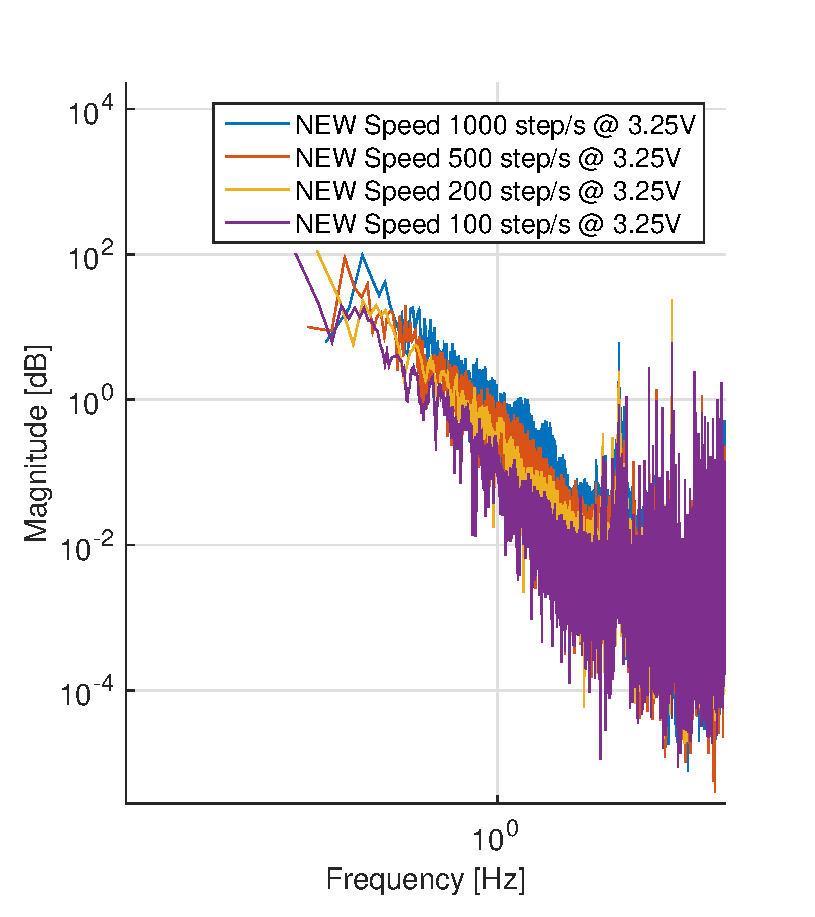
\includegraphics[width=0.46\textwidth, trim=0cm 0cm 0.8cm 0cm, clip=true]{fig/matlab/differentspeeds2.eps}}
  \qquad
  \subfloat[][\label{fig:dist_diff_speed_zoomin}Zoom-in]{
  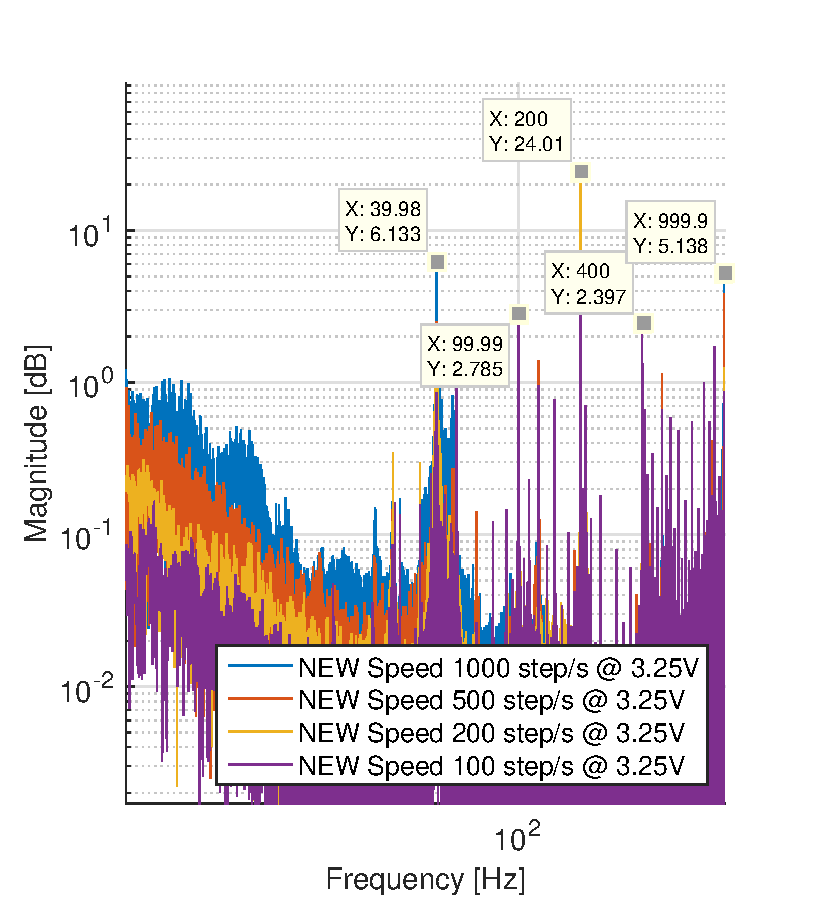
\includegraphics[width=0.46\textwidth, trim=0cm 0cm 0.8cm 0cm, clip=true]{fig/matlab/differentspeeds_Zoomin2.eps}}
  \caption{\label{fig:dist_diff_speed} \abbrFFT of the yaw angle in open loop with the rotational head in 0 mrad (3.25V). The whole spectrum is shown in (a) while a zoom-in is shown in (b). One can see how the induced harmonics are multiples of the stepping speeds.}
\end{figure}

\newpage
\FloatBarrier
\section{Model Reference Adaptive Control}
Even though the rotational stage has been modeled by \eqref{eq:tf}, a second order model approximating the higher order system was used in the adaptive control laws to keep the computational burden low. The discretized reference model can be seen in \eqref{eq:sys_gm} and all parameters and tuning variables are summarized in Table~\ref{tab:adaptive_param}. The controller was tuned to be robust to input disturbances and model changes. The set of parameter presented in Table~\ref{tab:adaptive_param} is not an optimal set but a decent set of parameters that maintains stability for step sizes below 20mrad.

\begin{equation}
  \label{eq:sys_gm}
  G_m(z) = \frac{7.9z + 6.7}{1313z^{2} - 2095z + 796.4}
\end{equation}

\begin{table}[h!]
  \centering
  \begin{tabular}{| l | l |}
    \hline
    Parameter & Value \\ \hline
    $T_s$ & $5 \times 10^{-4}$ \\
    $\alpha_0$ & $5.7 \times 10^{4}$ \\
    $\alpha_1$ & $7.2$ \\
    $\beta_0$ & $7.5 \times 10^{7}$ \\
    $a_0$ & $5.7 \times 10^{4}$ \\
    $a_1$ & $1 \times 10^{3}$ \\
    $b_0$ & $7.5 \times 10^{7}$ \\
    $\eta_0$ & $3 \times 10^{-2}$ \\
    $\eta_1$ & $1 \times 10^{-1}$ \\
    $\eta_2$ & $1 \times 10^{-10}$ \\
    $\eta_3$ & $1 \times 10^{-17}$ \\
    $\epsilon$ & $1 \times 10^{-8}$ \\
    $Q$ & $diag(1 \times 10^{10}, 1 \times 10^{-3})$\\
    \hline
  \end{tabular}
  \caption{\label{tab:adaptive_param} Parameters of the system model and the tuned adaptive controller.}
\end{table}

Figure~\ref{fig:step_adaptive} shows the step response to different step sizes. Here it is clear that the system becomes unstable if the step size $\geq$ \unit{26}{\milli\radian}. Note that all tests were produced with initial values $k_i = 0$.

\begin{figure}[h!]
  \centering
  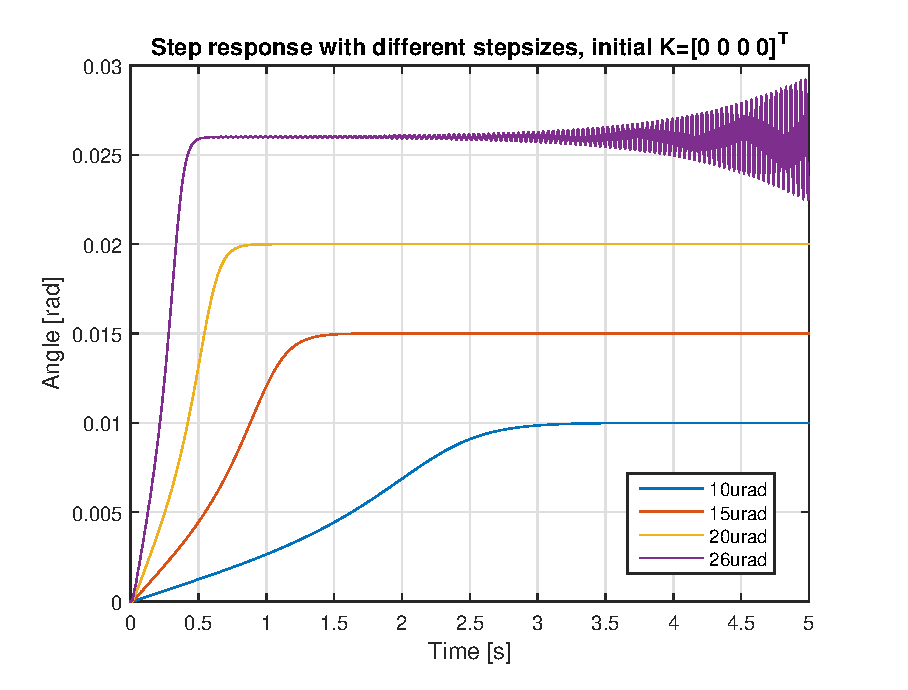
\includegraphics[width=0.7\textwidth]{fig/matlab/stepresponse.eps}
  \caption{\label{fig:step_adaptive} Step responses to step sizes of 10, 15, 20 and 26 mrad.}
\end{figure}

The adaptation process of the control parameters $k_i$, for a step response resulting from a 20mrad step, can be seen in Figure~\ref{fig:adapt_process}. All of the coefficients have converged within 1 second.

\begin{figure}[h!]
  \centering
  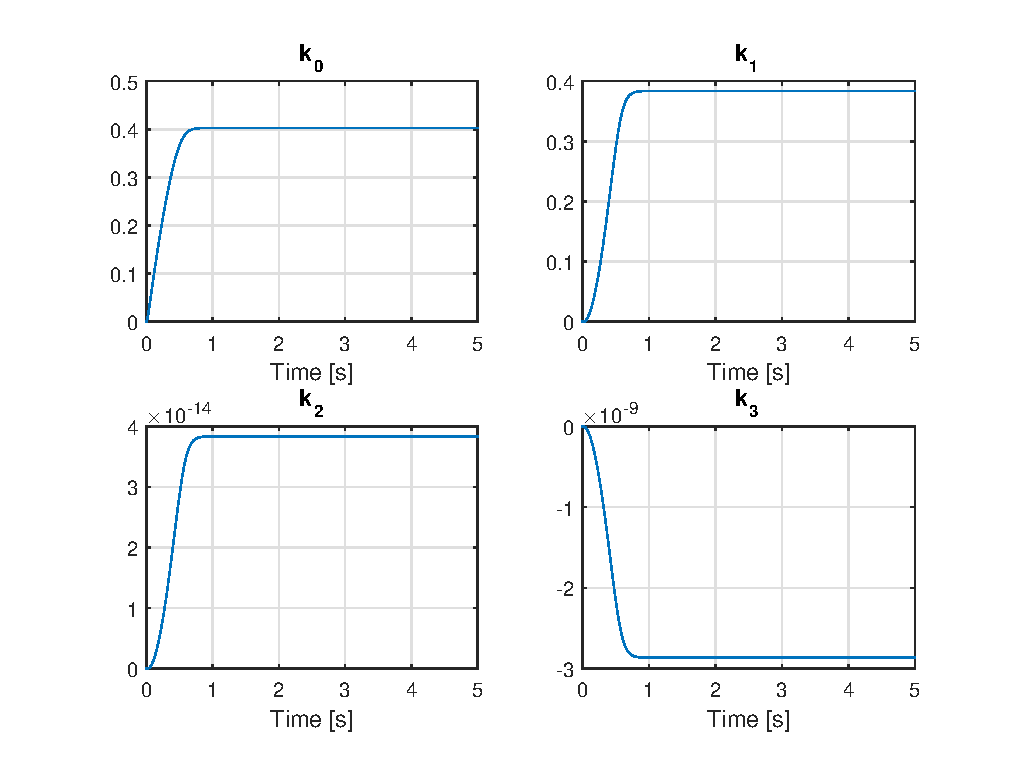
\includegraphics[width=1\textwidth]{fig/matlab/k.eps}
  \caption{\label{fig:adapt_process} Adaptation process of control parameters $k_i$ with a 20 mrad step.}
\end{figure}

\FloatBarrier
To illustrate the adaptation process better, a periodic response is depicted in Figure~\ref{fig:periodic_resp} which shows that after the adaptation process is finished the controller performs better for the second and third period. One can see that the adaptation process is slower for the periodic response corresponding to a lower step. Hence, the lower the step, the longer the adaptation time. The present controller tracks the periodic input well independently of the step size.

\begin{figure}[h!]
  \centering
  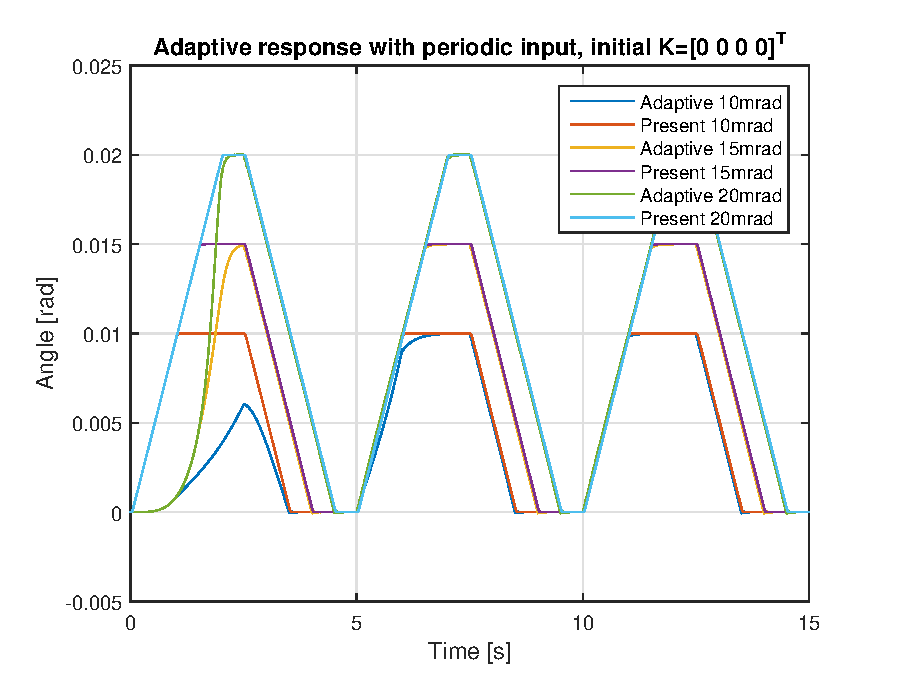
\includegraphics[width=0.7\textwidth]{fig/matlab/periodicresponse.eps}
  \caption{\label{fig:periodic_resp} Periodic responses for the adaptive and present controller with amplitudes of 10, 15, 20 mrad.}
\end{figure}

\begin{figure}[h!]
  \centering
  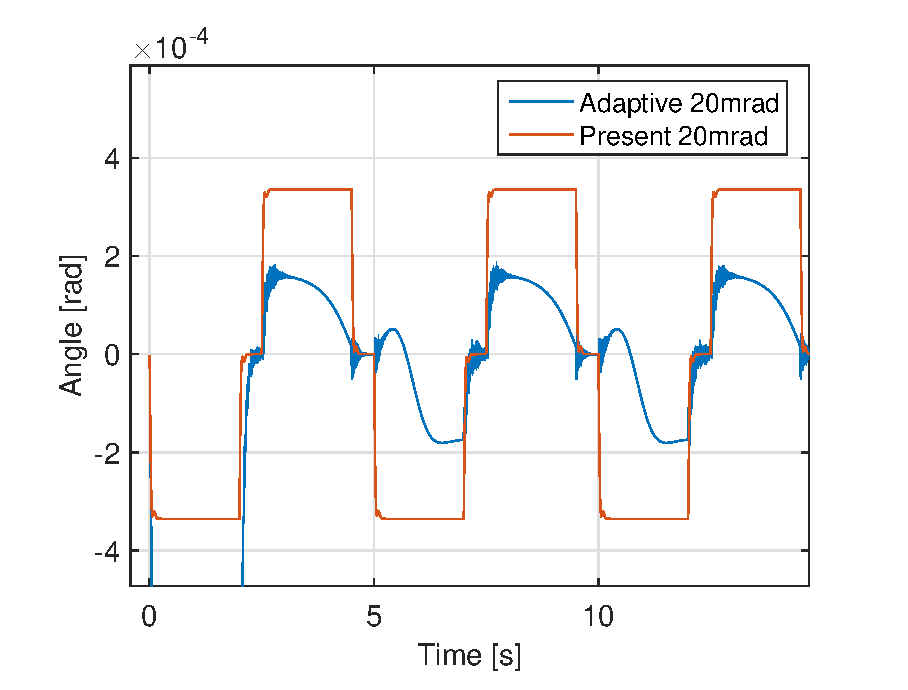
\includegraphics[width=0.7\textwidth]{fig/matlab/trackingerror.eps}
  \caption{\label{fig:adapt_trackingerror} Tracking error (difference between reference and output) for the periodic response from an input signal with an amplitude of 20 mrad.}
\end{figure}

The tracking error corresponding to the \emph{Adaptive 20mrad} and \emph{Present 20mrad} in Figure~\ref{fig:periodic_resp} can be seen in Figure~\ref{fig:adapt_trackingerror}. The adaptive controller performs better than the present controller after the adaptation process has finished.

A periodic response with model parameter drift is presented in Figure~\ref{fig:modeldrift}. It shows how the adaptive controller manages to adapt to changes in the system dynamics, while the present controller fails to do so, resulting in an unstable system. The change of the model was performed over 2 seconds, resulting in a movement of the first resonance peak, from 38 Hz to 66 Hz in frequency and from 30.1 dB to 23.5 dB in magnitude.
\begin{figure}[h!]
  \centering %crop: left bottom right top
  \subfloat[][\label{fig:modeldriftresponse}Periodic response with model parameter drift.]{
  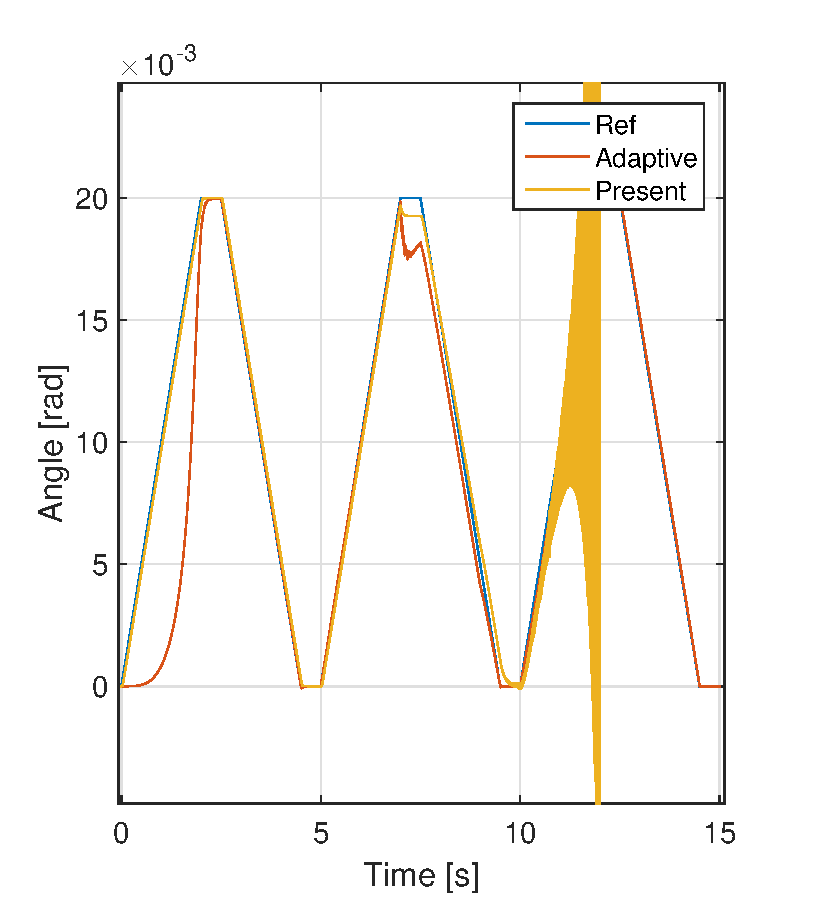
\includegraphics[width=0.46\textwidth, trim=0cm 0cm 1cm 0cm, clip=true]{fig/matlab/driftofmodelparameterover2s.eps}}
  \qquad
  \subfloat[][\label{fig:modeldriftbode}Original model (G) and the resulting model after drift ($G_{mod}$).]{
  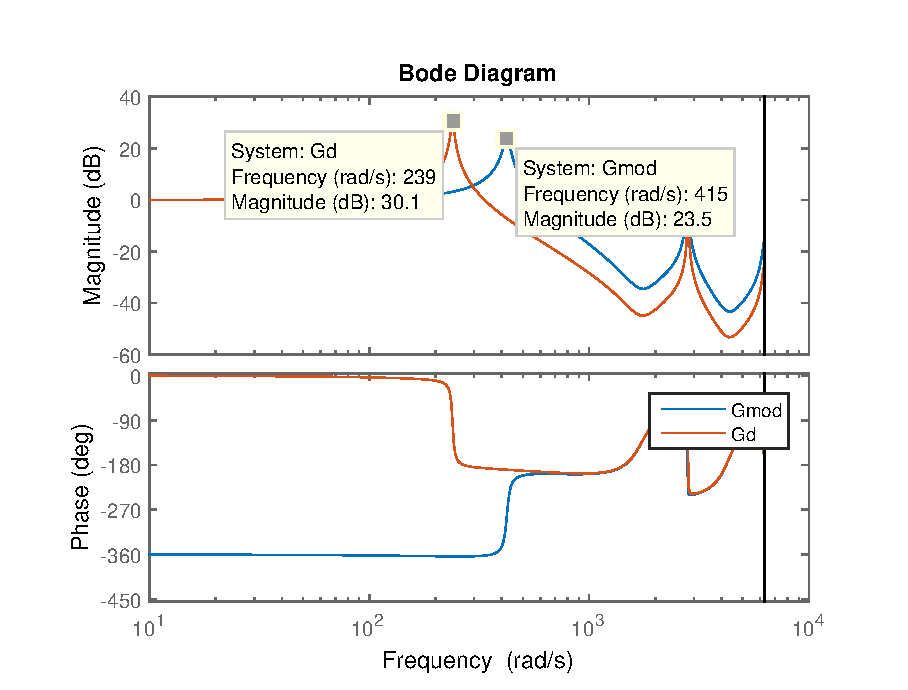
\includegraphics[width=0.46\textwidth, trim=0cm 0cm 0.7cm 0cm, clip=true]{fig/matlab/bode_drift_pole.eps}}
  \caption{\label{fig:modeldrift} Shows the robustness to model changes over time. The model error is increased linearly from $t=7s$ to $t=9s$. The resulting responses are shown in (a) with the model change in (b).}
\end{figure}

\begin{figure}[h!]
  \centering %crop: left bottom right top
  \subfloat[][\label{fig:modelerrorresponse}Periodic response with model parameter drift.]{
  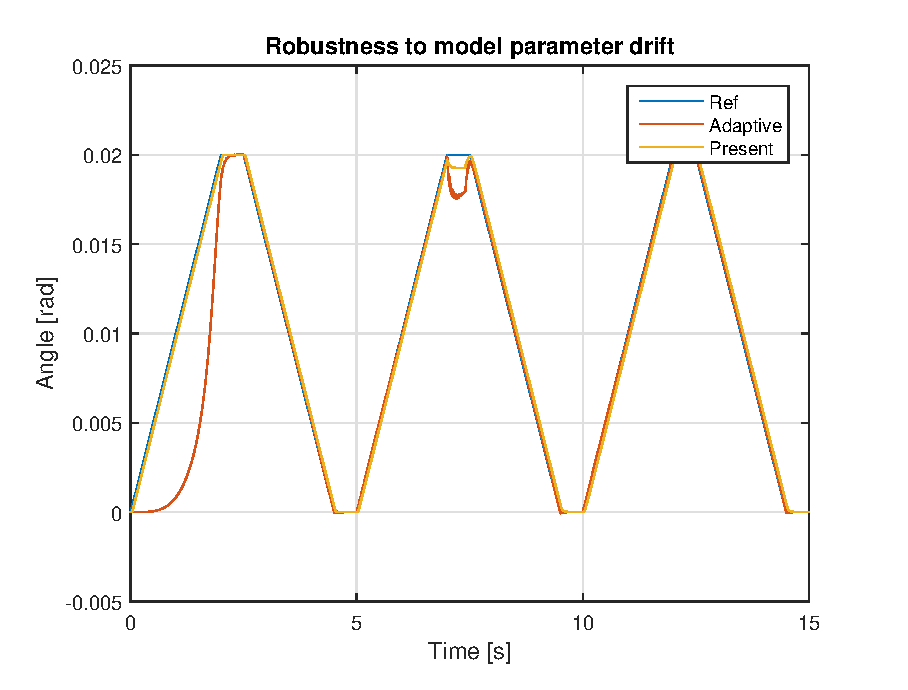
\includegraphics[width=0.46\textwidth, trim=0cm 0cm 1cm 0cm, clip=true]{fig/matlab/modelerrorperiodic.eps}}
  \qquad
  \subfloat[][\label{fig:modelerrorbode}Original model (G) and the resulting model after drift ($G_{mod}$).]{
  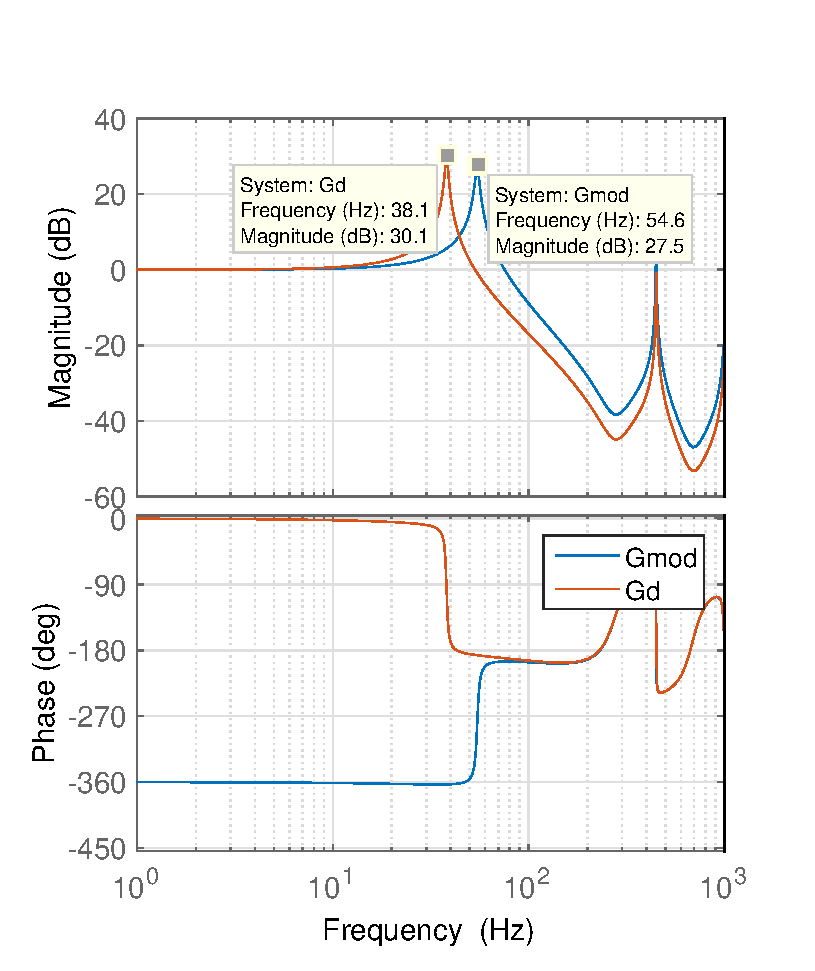
\includegraphics[width=0.46\textwidth, trim=0cm 0cm 0.7cm 0cm, clip=true]{fig/matlab/bode_modelerror_pole.eps}}
  \caption{\label{fig:modelerror}Robustness to model changes over time. The model error is increased linearly from $t=5s$ to $t=7s$. The resulting responses are shown in (a) with the model change in (b).}
\end{figure}

In the case in Figure~\ref{fig:modelerror} the resonance peak is only moved by 17 Hz and the present controller is sufficient to suppresses the disturbance. It even does it more efficiently than the adaptive controller. Even though the adaptive controller is slower than the present controller it still achieves a smaller tracking error after the adaption process is over, see Figure~\ref{fig:modelerror_trackingerror}. Note that the change in the model is equivalent to the change between 0V and 6.5V presented in Figure~\ref{fig:different_angles}.

\begin{figure}[h!]
  \centering
  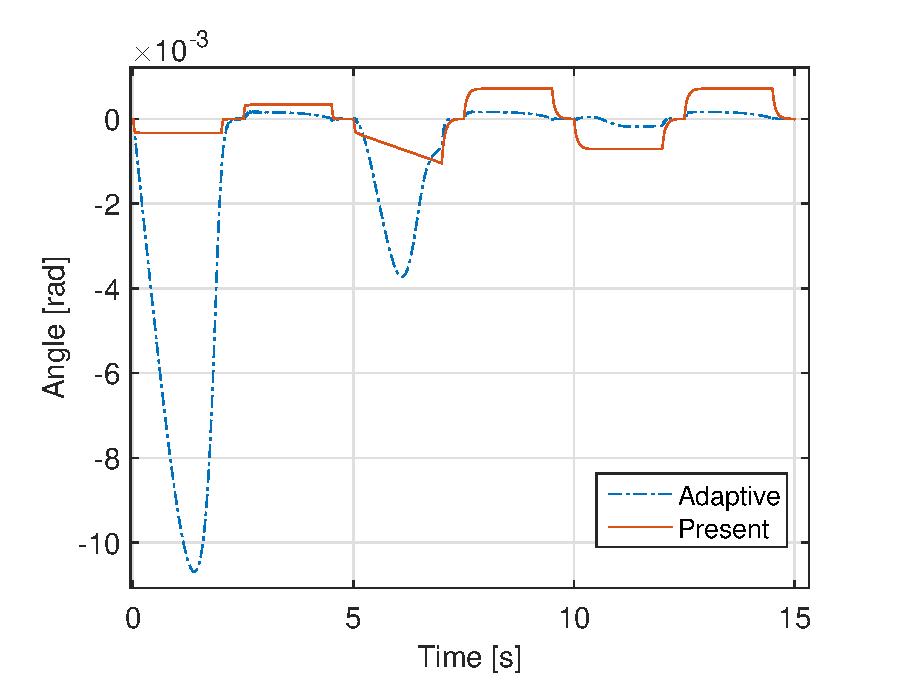
\includegraphics[width=0.7\textwidth]{fig/matlab/modelerrorperiodic_trackingerror.eps}
  \caption{\label{fig:modelerror_trackingerror} Tracking error for the periodic response with a model error drift from $t=5s$ to $t=7s$.}
\end{figure}

\FloatBarrier
Figure~\ref{fig:distrejection} and \ref{fig:distmeasrejection} shows the disturbance rejection capability to a disturbance applied on the input and output of the system. In Figure~\ref{fig:distrejection} a small impulse was added to the input. The adaptive controller performed worse than the present controller. The present controller managed to attenuate the highest peak of the impulse by 1.5 times more than the adaptive. The settling time was also approximately 3 times worse for the adaptive controllers. In Figure~\ref{fig:distmeasrejection} the impulse was instead added to the output of the system. Even in this case the present controller was superior, attenuating the highest peak of the impulse by 3 times more than the adaptive controller.

\begin{figure}[h!]
  \centering %crop: left bottom right top
  \subfloat[][\label{fig:dist}Step response]{
  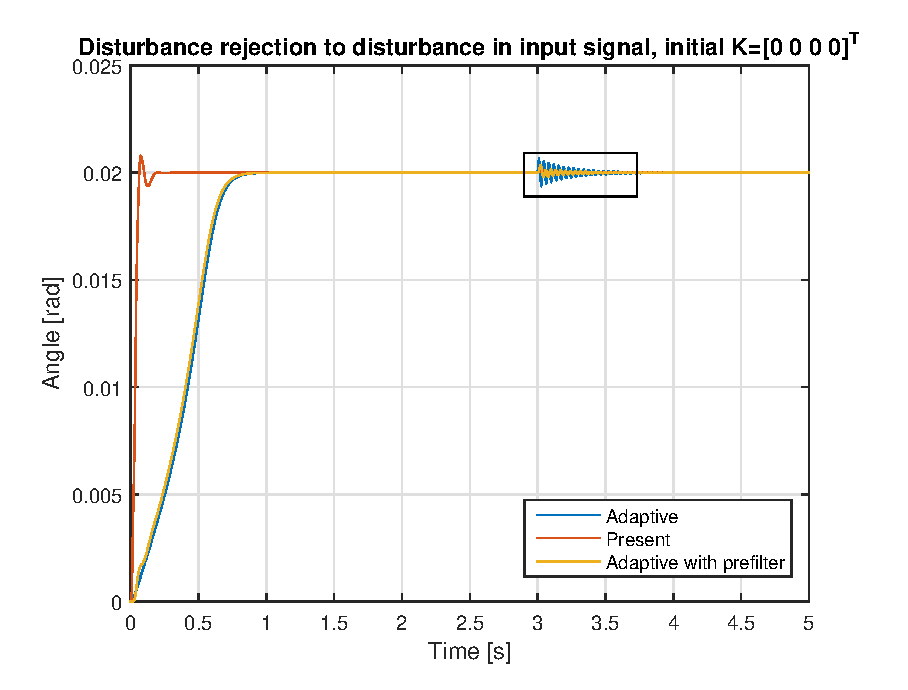
\includegraphics[width=0.46\textwidth, trim=0cm 0cm 1cm 0.8cm, clip=true]{fig/matlab/distrejection.eps}}
  \qquad
  \subfloat[][\label{fig:distzoom}Zoom-in on disturbance]{
  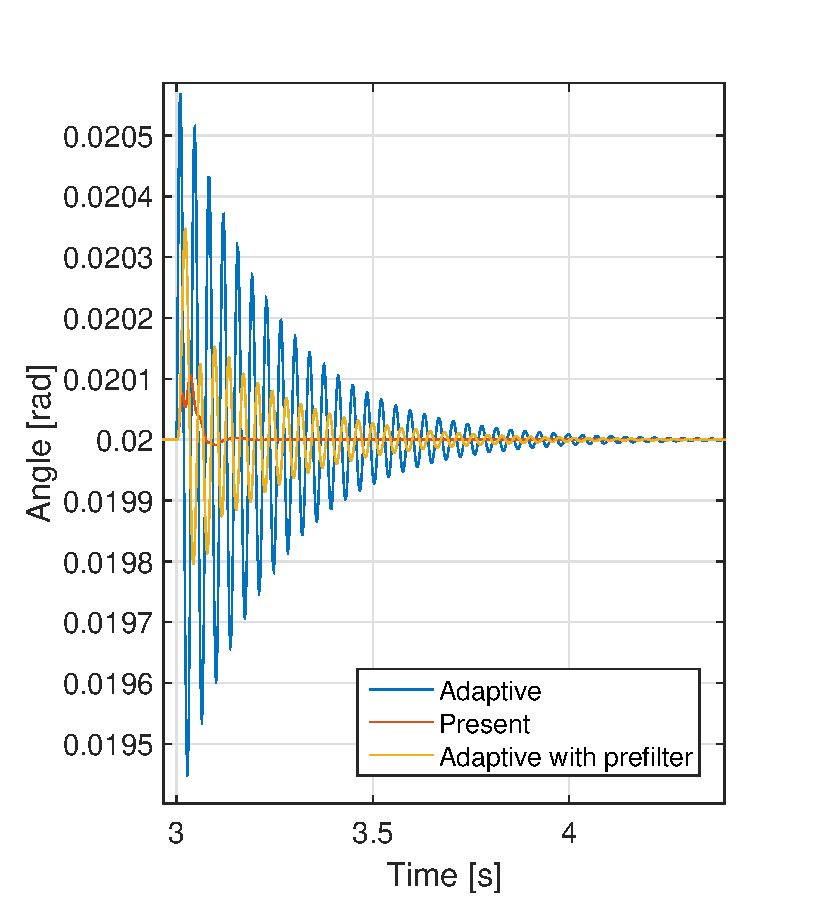
\includegraphics[width=0.46\textwidth, trim=0cm 0cm 1cm 0.8cm, clip=true]{fig/matlab/distrejection_zoom.eps}}
  \caption{\label{fig:distrejection} Controller attenuation of a disturbance impulse (amplitude of $5.1 \times 10^{-3}$) added to the input signal at $t=3s$. The whole step response is shown in (a) with a zoom-in on the disturbance in (b).}
\end{figure}
\begin{figure}[h!]
  \centering %crop: left bottom right top
  \subfloat[][\label{fig:distmeas}Step response]{
  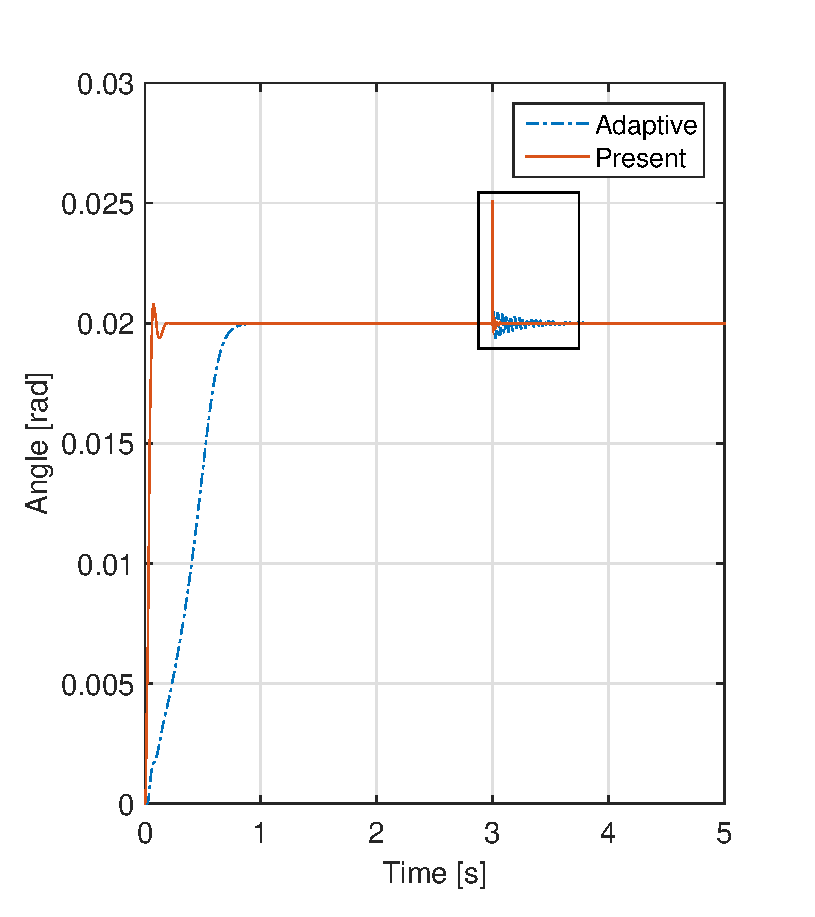
\includegraphics[width=0.46\textwidth, trim=0cm 0cm 1cm 0.8cm, clip=true]{fig/matlab/distrejection_meas.eps}}
  \qquad
  \subfloat[][\label{fig:distmeaszoom}Zoom-in on disturbance]{
  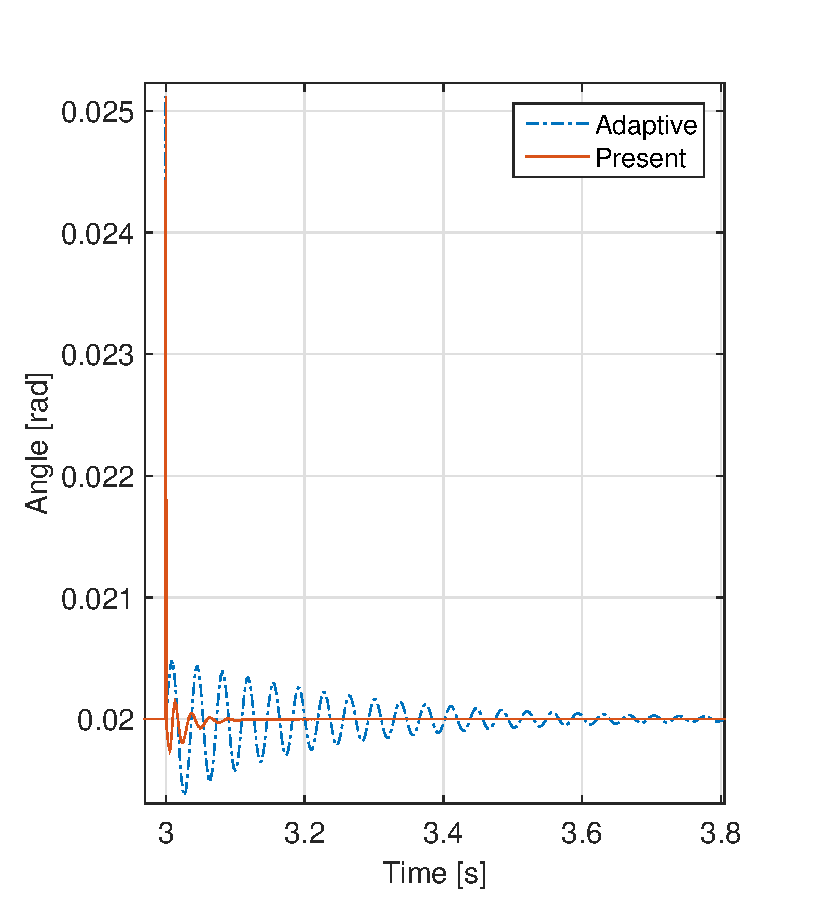
\includegraphics[width=0.46\textwidth, trim=0cm 0cm 1cm 0.8cm, clip=true]{fig/matlab/distrejection_meas_zoom.eps}}
  \caption{\label{fig:distmeasrejection} Disturbance rejection to impulses (amplitude of $5.1 \times 10^{-3}$) added to the measured signal at $t=3s$. The step response is shown in (a)  with a zoom-in on the disturbance in (b).}
\end{figure}

\newpage~\newpage~
\FloatBarrier
\section{Integral Resonance Control}
The \abbrIRC's design procedure presented in \ref{sec:irc} was carried out in continuous time, but each block in the scheme was individually discretized for the sake of comparison with the present controller. The continuous time representation of the system in \eqref{eq:tf} contains 7 poles and 6 zeros i.e. a relative degree of 1. A negative feedforward would therefore introduce another zero that can be placed in a desired position by adjusting the gain $D_f$. As seen in the pole-zero plot comparison in Figure~\ref{fig:negfeedpzmap}, a feedforward of $D_f=-1.2$ was sufficient to introduce one zero and place it and its complex conjugate below the first resonance frequency. This and the zero-pole interlacing for the higher order modes can be seen in Figure~\ref{fig:pzafter}, where the zoom-in shows the complex conjugate zeros below the first resonance mode.

\begin{figure}[h!]
  \centering %crop: left bottom right top
  \subfloat[][\label{fig:pzbefore}Origianl system]{
  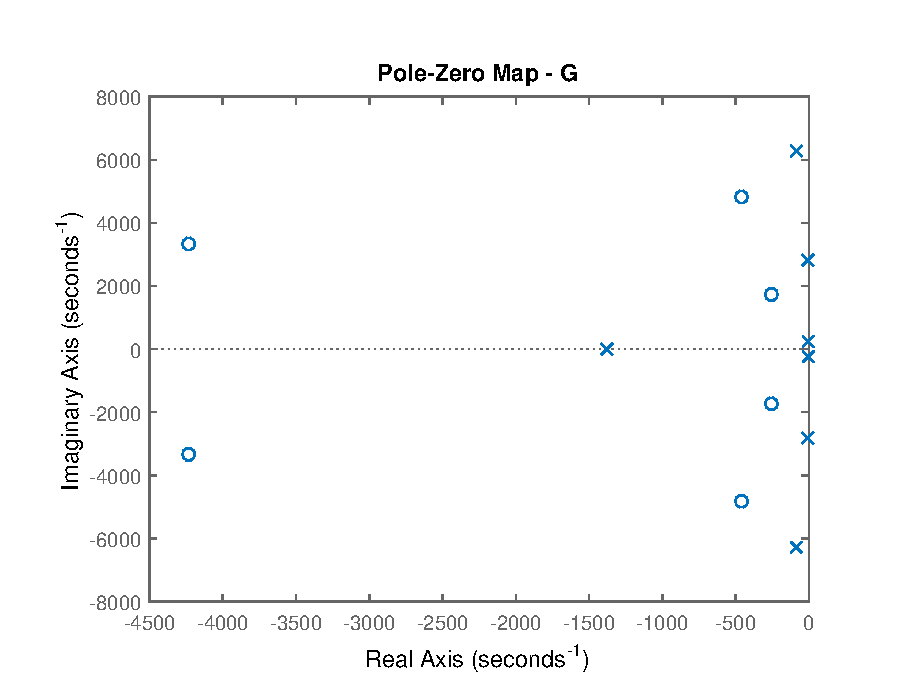
\includegraphics[width=0.46\textwidth, trim=0cm 0cm 1cm 0cm, clip=true]{fig/matlab/pzbefore.eps}}
  \qquad
  \subfloat[][\label{fig:pzafter}After feedforward]{
  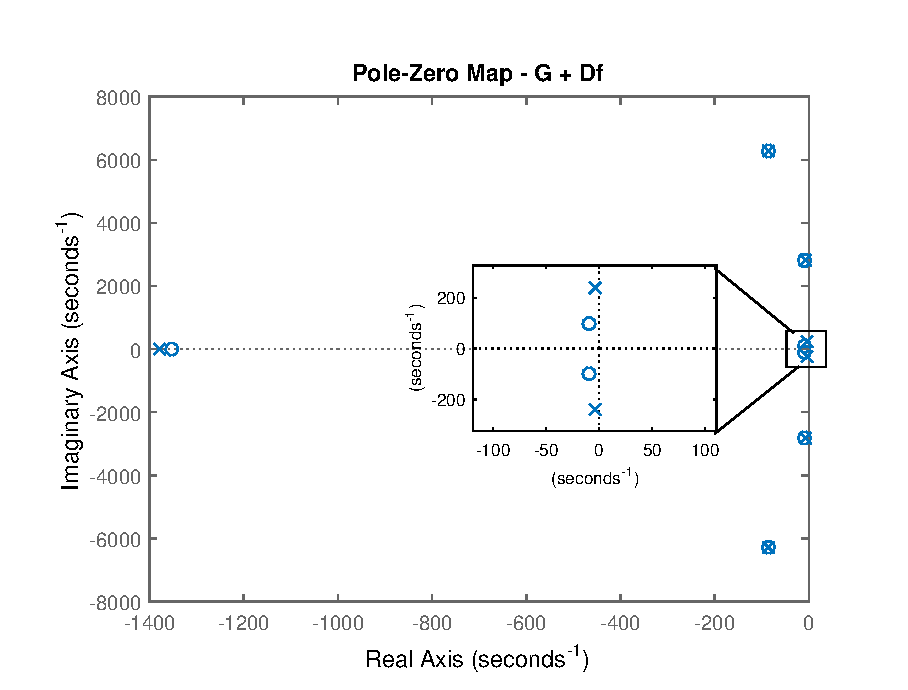
\includegraphics[width=0.46\textwidth, trim=0cm 0cm 1cm 0cm, clip=true]{fig/matlab/pzafter.eps}}
  \caption{\label{fig:negfeedpzmap} Comparison of pole-zero plot before and after adding the negative feedforward. After adding the feedforward to the system which poles and zeros are shown in (a) , the zeros and poles are interlacing as seen in (b).}
\end{figure}
\FloatBarrier
The corresponding Bode plot can be seen in Figure~\ref{fig:bodeafterfeedf}, showing the complex conjugate pair of zeros as a dip before the first resonance peak.

\begin{figure}[h!]
  \centering
  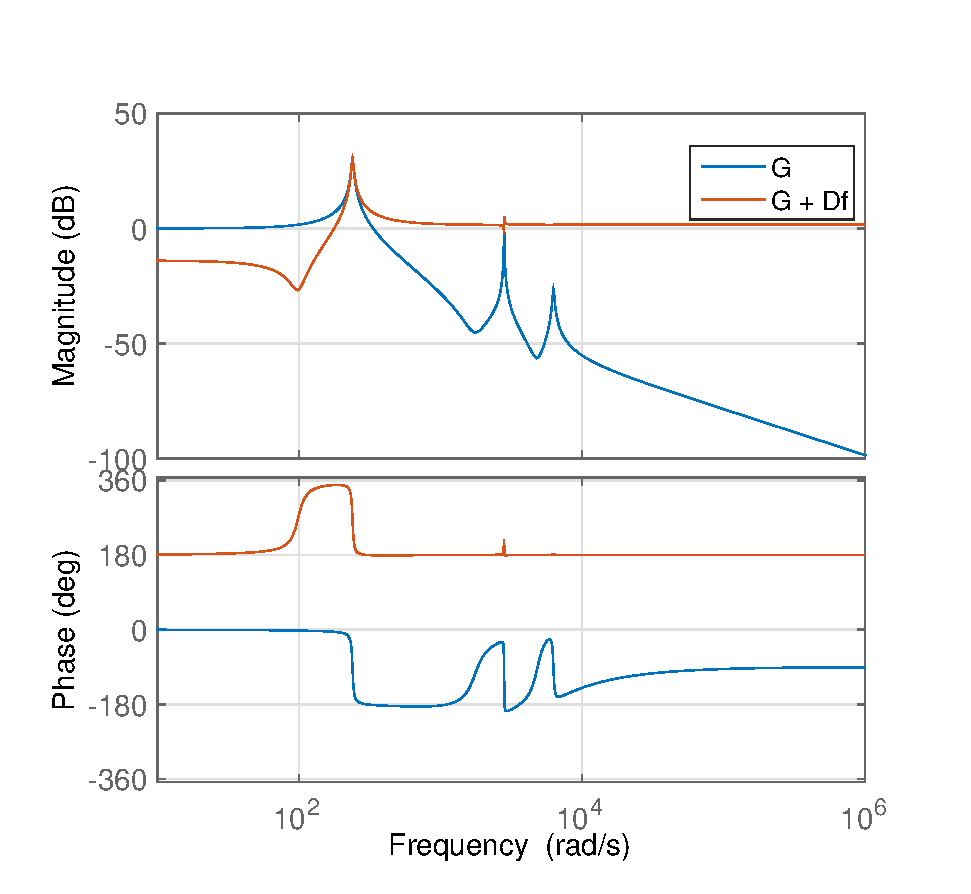
\includegraphics[width=0.7\textwidth]{fig/matlab/bodeafterfeedf.eps}
  \caption{\label{fig:bodeafterfeedf} Bode plot of the system before and after the addition of the negative feedforward.}
\end{figure}

\FloatBarrier
The integral controller $C=\frac{-k}{s}$ was added according to Section~\ref{sec:irc} and a gain of $k=314$ was found to maximize the damping, by using the root locus technique.
The open and closed loop system of the \abbrIRC damping loop depicted in Figure~\ref{fig:irc} is shown in Figure~\ref{fig:bodedamped}. It is clear that the integral controller damps out the first resonance peak efficiently in closed loop.

\begin{figure}[h!]
  \centering
  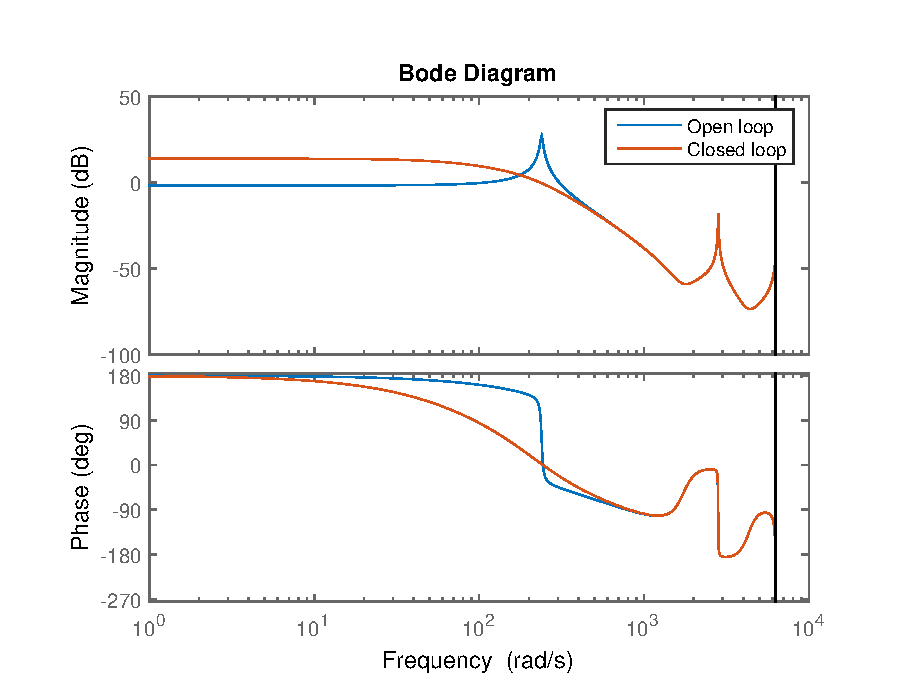
\includegraphics[width=0.7\textwidth]{fig/matlab/bodedamped.eps}
  \caption{\label{fig:bodedamped} Open and closed loop of the \abbrIRC damping loop.}
\end{figure}

Finally, the damped system was enclosed in an outer loop with a second controller $C_1$ for reference tracking capability. $C_1$ was designed to be robust to model errors i.e. keep the sensitivity function $G_{dy}$ stated in \eqref{eq:Gyd} low for the frequencies that the model changes with (d and y in $G_{dy}$ can be found in the block scheme in Figure~\ref{fig:irc_int}). It was also designed to attenuate higher order resonances by including a notch filter.  $C_1$ was designed in Matlab's SISO-Tool and is presented in \eqref{eq:C_1}.

\begin{equation}
  \label{eq:Gyd}
  G_{yd} = \frac{1}{1 + C_2G(1 + C_1)}
\end{equation}

\begin{equation}
  \label{eq:C_1}
  C_1 = \frac{-13.54 z^5 + 40.92 z^4 - 57.47 z^3 + 55.89 z^2 - 35.87 z + 10.05}{z^5 - 1.65 z^4 + 0.80 z^3 - 0.16 z^2 + 0.014 z - 0.00042}
\end{equation}

The resulting closed loop system and the sensitivity function is shown in Figure~\ref{fig:irc_totalclosed} and \ref{fig:sensitivity_irc}, respectively. The plots show that the use of the \abbrIRC has increased the closed loop bandwidth from 11 Hz to 73 Hz, corresponding to an increase of 6.5 times the present closed loop bandwidth.

\begin{figure}[h!]
  \centering
  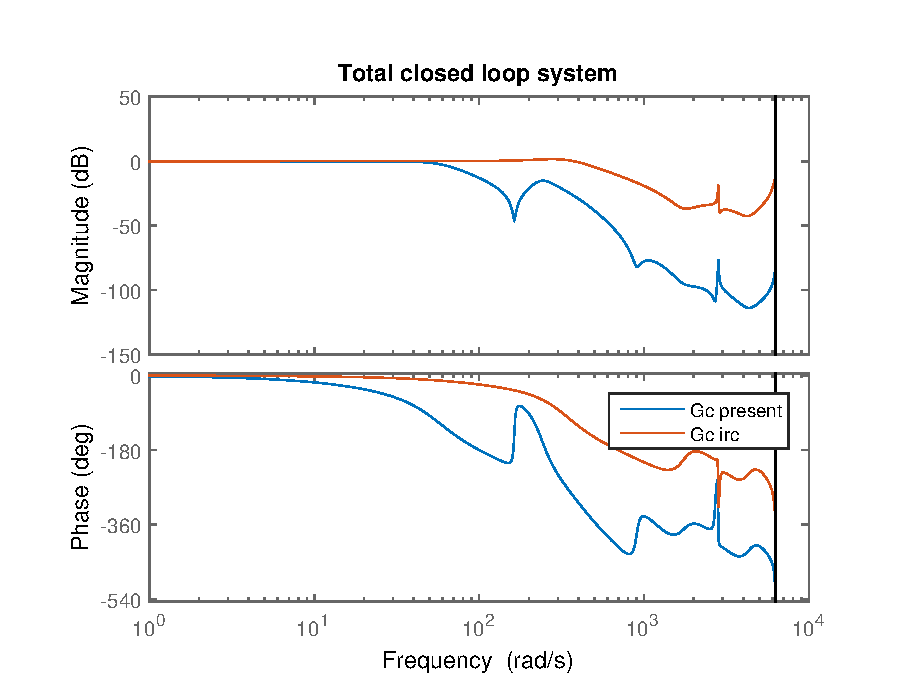
\includegraphics[width=0.7\textwidth]{fig/matlab/totalclosedloop.eps}
  \caption{\label{fig:irc_totalclosed} Closed loop system of the \abbrIRC and the present approach}
\end{figure}

The \abbrIRC's sensitivity function also shows that the \abbrIRC scheme attenuates model disturbances better in the low frequency range and in the region within 24-64 Hz.

\begin{figure}[h!]
  \centering
  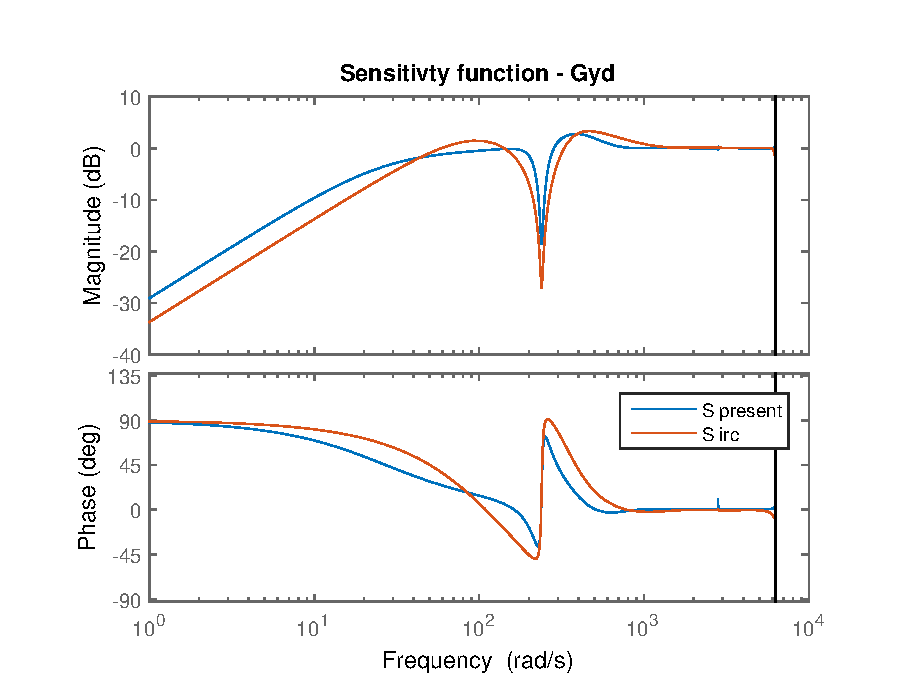
\includegraphics[width=0.7\textwidth]{fig/matlab/sensitivity_irc.eps}
  \caption{\label{fig:sensitivity_irc}Sensitivity function ($G_{dy}$) of the \abbrIRC and the present approach}
\end{figure}

\FloatBarrier
The \abbrIRC's tracking performance is shown in Figure~\ref{fig:irc_tracking}, which has reduced the tracking error considerably due to its high bandwidth.

\begin{figure}[h!]
  \centering %crop: left bottom right top
  \subfloat[][\label{fig:irc_periodic}Periodic Response]{
  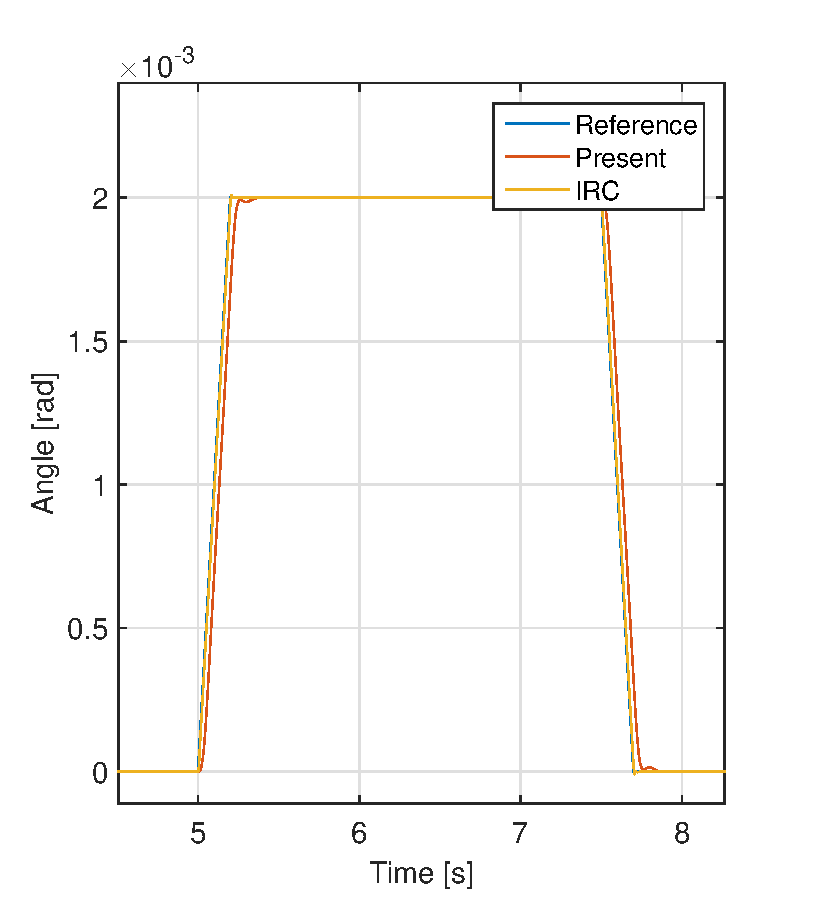
\includegraphics[width=0.46\textwidth, trim=0cm 0cm 1cm 0cm, clip=true]{fig/matlab/irc_periodic.eps}}
  \qquad
  \subfloat[][\label{fig:irc_tracking_error}Tracking error]{
  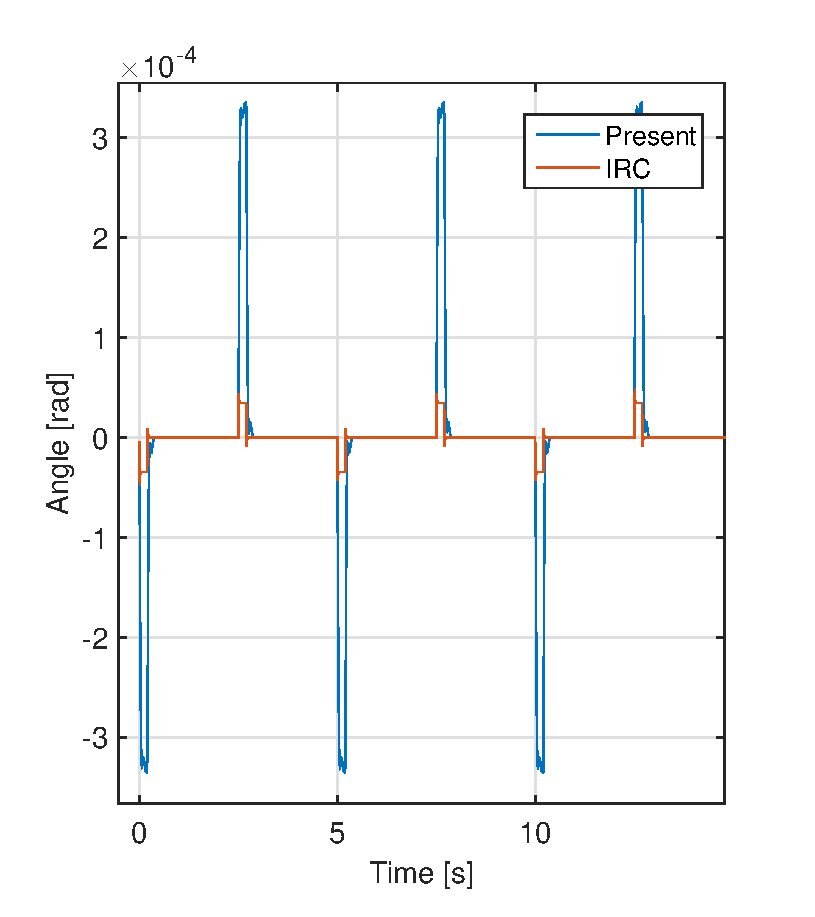
\includegraphics[width=0.46\textwidth, trim=0cm 0cm 1cm 0cm, clip=true]{fig/matlab/irctrackingerror.eps}}
  \caption{\label{fig:irc_tracking} A zoom on one period of the periodic response is shown in (a) while the tracking error over three periods are shown in (b).}
\end{figure}

The robustness test performed for the adaptive controller was done for the \abbrIRC controller accordingly. Figure~\ref{fig:irc_dist_model} shows the periodic response and its tracking error when the model is changed linearly according to Figure~\ref{fig:modelerrorbode}. The \abbrIRC handles the model drift better than the present controller.

\begin{figure}[h!]
  \centering %crop: left bottom right top
  \subfloat[][\label{fig:irc_dist_model}Periodic response]{
  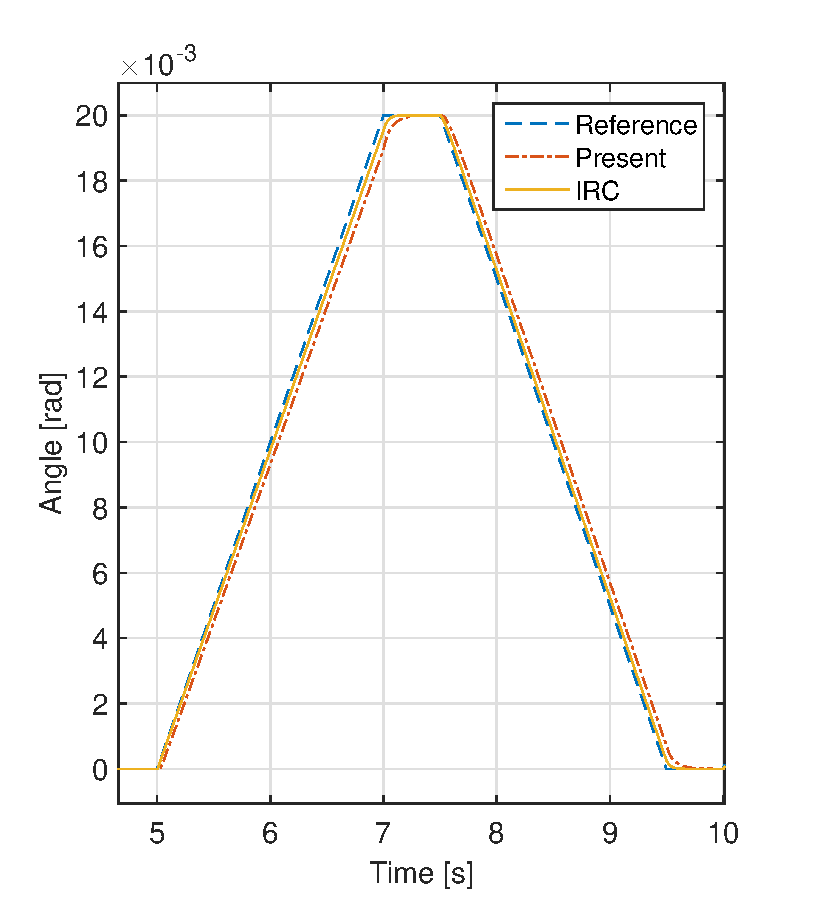
\includegraphics[width=0.46\textwidth, trim=0cm 0cm 1cm 0cm, clip=true]{fig/matlab/irc_periodic_drift.eps}}
  \qquad
  \subfloat[][\label{fig:irc_dist_model_drift}Periodic response with model parameter drift.]{
  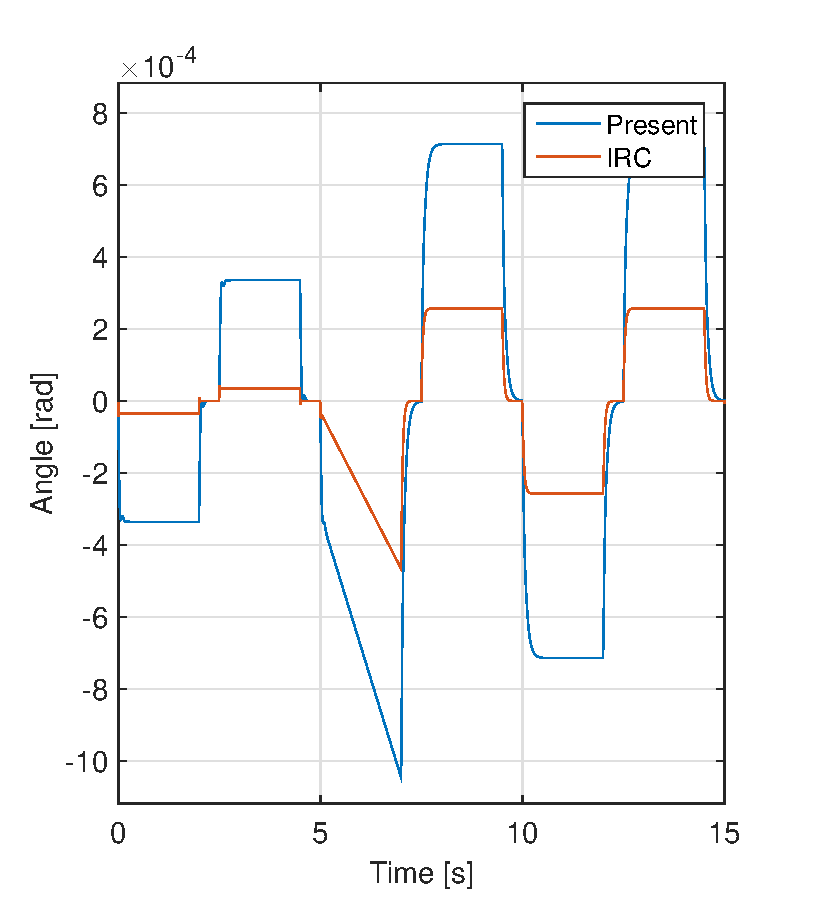
\includegraphics[width=0.46\textwidth, trim=0cm 0cm 1cm 0cm, clip=true]{fig/matlab/irc_periodic_trackingerror.eps}}
  \caption{\label{fig:irc_dist} Shows the robustness to model changes over time. The model error is increased linearly from $t=5s$ to $t=7s$.  A zoom-in on one period is shown in (a) while the tracking error over three periods are shown in (b).}
\end{figure}

\FloatBarrier
The \abbrIRC capability of rejecting disturbances on the input signal is shown in Figure~\ref{fig:irc_dist_input}. As seen in the zoom-in, the \abbrIRC is slightly more damped but has a high frequency ringing in 448Hz, the same frequency as the model's second resonance peak. This ringing is also showing in the present controller but is less dominant.

\begin{figure}[h!]
  \centering %crop: left bottom right top
  \subfloat[][\label{fig:irc_dist_input_step}Step response]{
  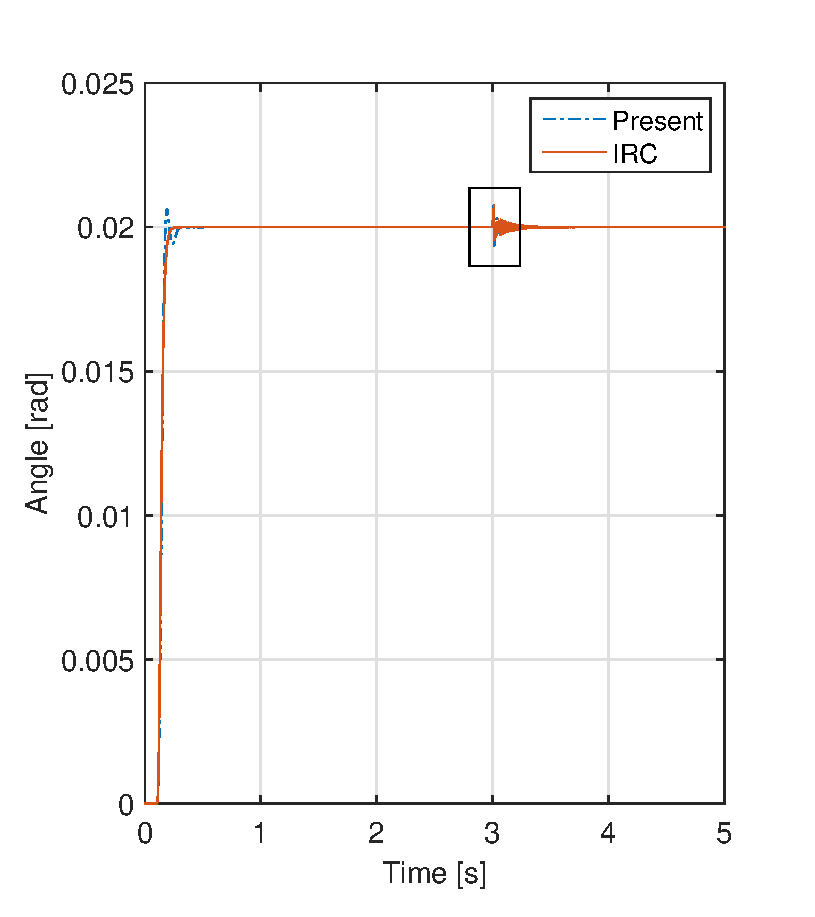
\includegraphics[width=0.46\textwidth, trim=0cm 0cm 1cm 0cm, clip=true]{fig/matlab/irc_dist_input.eps}}
  \qquad
  \subfloat[][\label{fig:irc_dist_input_zoom}Zoom-in on disturbance]{
  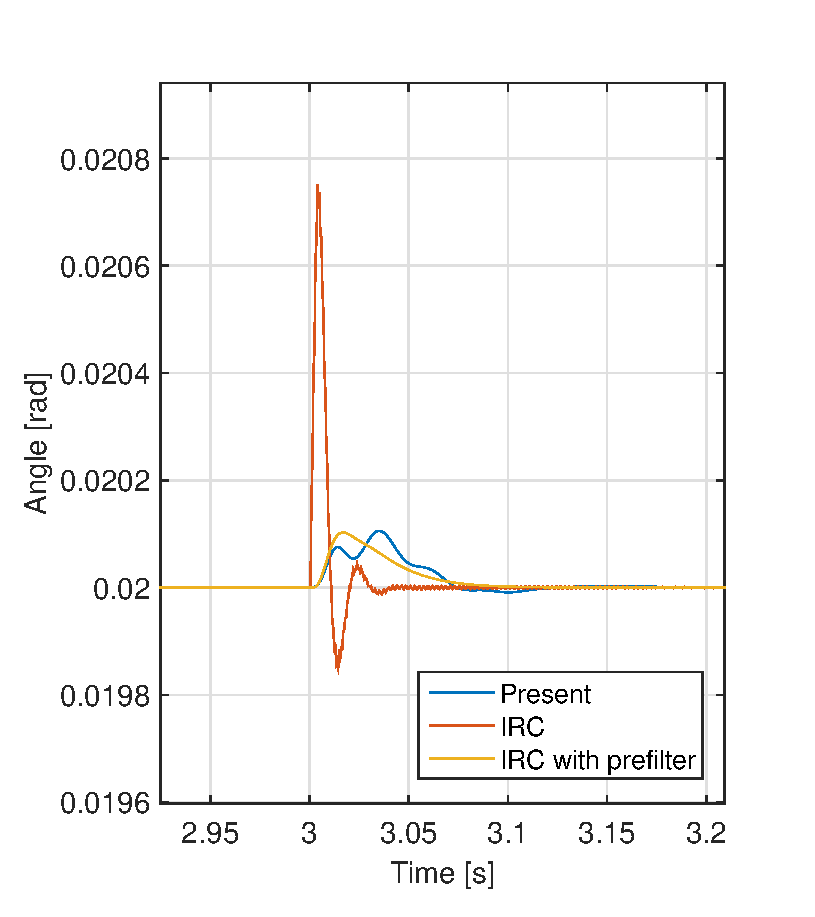
\includegraphics[width=0.46\textwidth, trim=0cm 0cm 1cm 0cm, clip=true]{fig/matlab/irc_dist_input_zoom.eps}}
  \caption{\label{fig:irc_dist_input} Shows how well the controller attenuates a disturbance impulse (amplitude of $5.1 \times 10^{-3}$) added to the input signal at $t=3s$. The whole step response is shown in (a) with a zoom-in on the disturbance in (b).}
\end{figure}

The \abbrIRC's capability of rejecting disturbances on the output signal is shown in Figure~\ref{fig:irc_dist_output}. Since the impulse is added directly on the output the steps response peaks accordingly at $t=3s$. It is hard to tell from Figure~\ref{fig:irc_dist_output_zoom}, but the peak is visible for both of the control approaches. After the peak, the methods perform similarly but with a higher damping of the low frequency mode for the \abbrIRC oscillations as shown in the zoom-in.

\begin{figure}[h!]
  \centering %crop: left bottom right top
  \subfloat[][\label{fig:irc_dist_output_step}Step response]{
  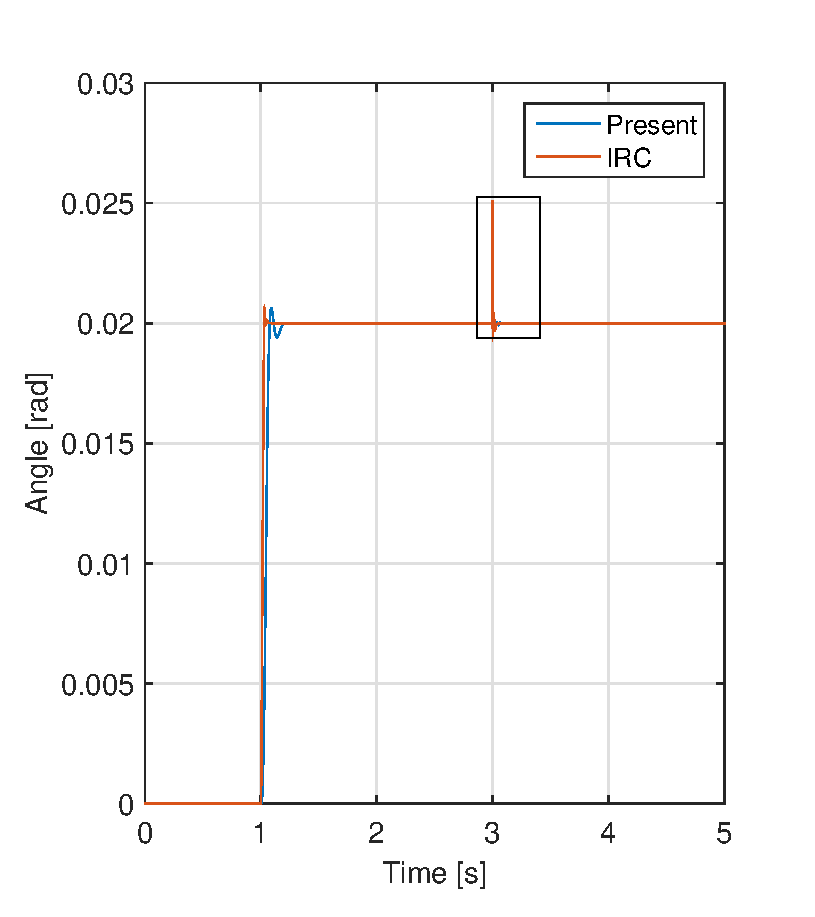
\includegraphics[width=0.46\textwidth, trim=0cm 0cm 1cm 0cm, clip=true]{fig/matlab/distrej_meas.eps}}
  \qquad
  \subfloat[][\label{fig:irc_dist_output_zoom}Zoom-in on disturbance]{
  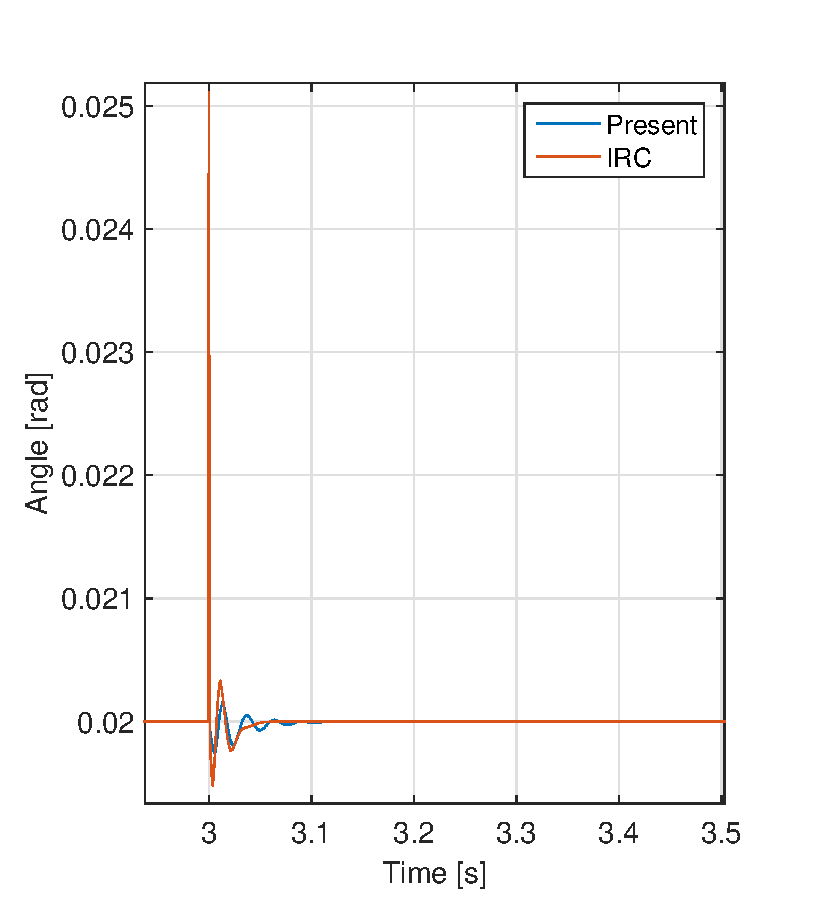
\includegraphics[width=0.46\textwidth, trim=0cm 0cm 1cm 0cm, clip=true]{fig/matlab/distrej_meas_zoom.eps}}
  \caption{\label{fig:irc_dist_output} Shows how well the controller attenuates a disturbance impulse (amplitude of $5.1 \times 10^{-3}$) added to the output signal at $t=3s$. The whole step response is shown in (a) with a zoom-in on the disturbance in (b).}
\end{figure}
\FloatBarrier
To further verify the controller capability of handling disturbances with various frequencies, a white noise was added to the input and output signal of the rotational stage ($G$), illustrated in Figure~\ref{fig:irc_int} as $d_i$ and $d_o$, respectively. The \abbrFFT was then performed on the output ($y$) to verify the disturbance rejection for all frequencies, and the result is presented in Figure~\ref{fig:fft_in} and Figure~\ref{fig:fft_out}.

\begin{figure}[h!]
  \centering
  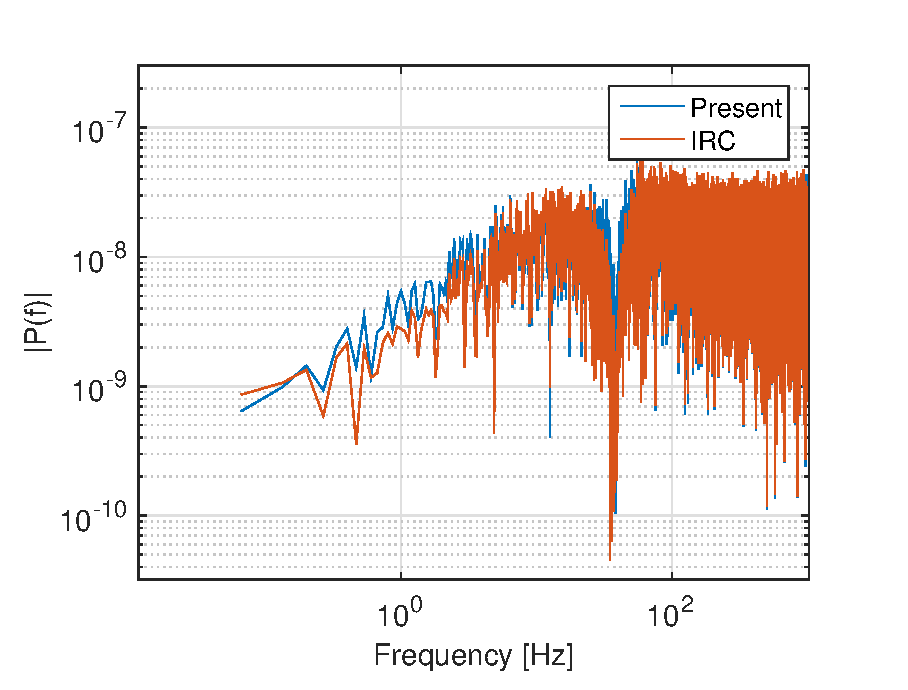
\includegraphics[width=0.7\textwidth]{fig/matlab/whitenoiseoutput.eps}
  \caption{\label{fig:fft_in} The \abbrFFT of the output signal for the \abbrIRC and the present approach, when applying a white noise to the input of G}
\end{figure}

\begin{figure}[h!]
  \centering
  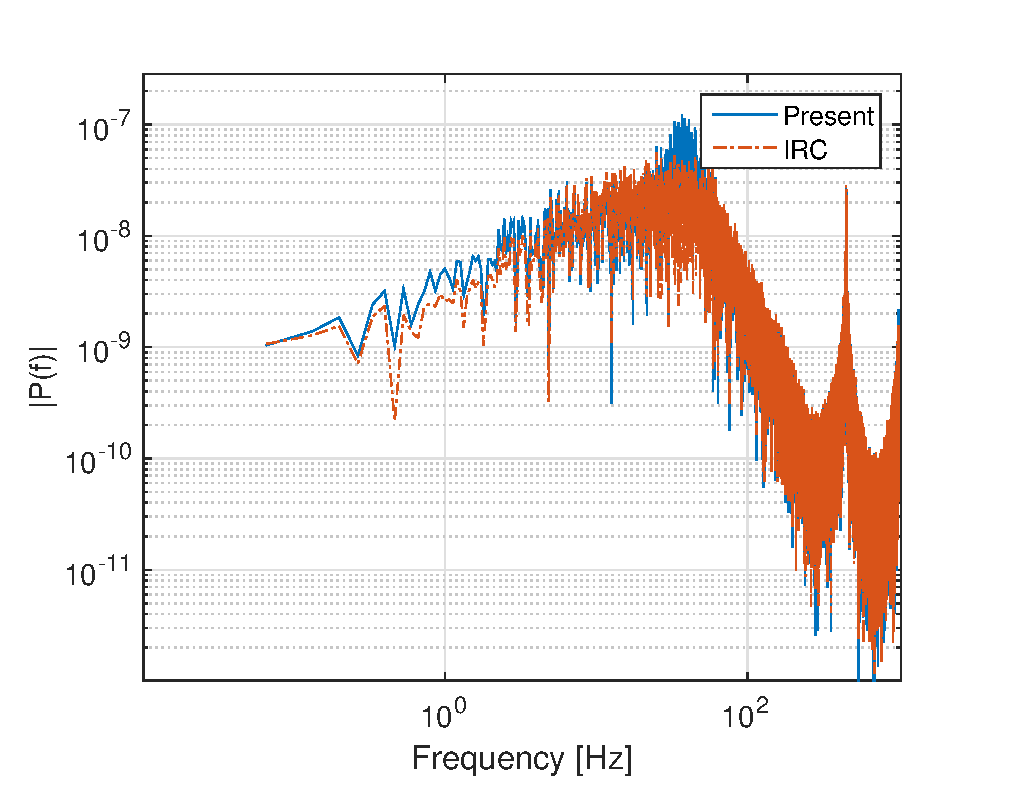
\includegraphics[width=0.7\textwidth]{fig/matlab/whitenoiseinput.eps}
  \caption{\label{fig:fft_out} The \abbrFFT of the output signal for the \abbrIRC and the present approach, when applying a white noise to the output of G}
\end{figure}


The standard deviations of the output signal with a disturbance with $\sigma$ = \unit{1.41\micro\radian} added to both the output and input for the \abbrIRC and the present approach are summarized in Table~\ref{tab:std}.

\begin{table}[h!]
  \centering
  \begin{tabular}{| l | l | l |}
    \hline
    Disturbance applied to: & input & output \\ \hline
      $\sigma_{Present}$ [\unit{\micro\radian}] & $0.68 $ & $1.43$ \\
      $\sigma_{IRC}$ [\unit{\micro\radian}] & $0.45$  & $ 1.46$ \\
    \hline
  \end{tabular}
  \caption{\label{tab:std} Standard deviations of the output signal}
\end{table}

Both approaches uses a static notch filter to cancel higher order harmonics, which makes the cancellation sensitive for model changes in the higher resonances. To benchmark the controller's robustness to these changes, a disturbance rejection test was performed. The system model was changed according to Figure~\ref{fig:high_model_error} where the highest resonance peak has been moved 83Hz and 97Hz while the controller was kept constant. The resulting response of a impulse applied to the output is presented in Figure~\ref{fig:model_dist_high_order}. The \abbrIRC is clearly more sensitive to model errors and becomes unstable when the highest resonance peak has moved by 97Hz.

\begin{figure}[h!]
  \centering
  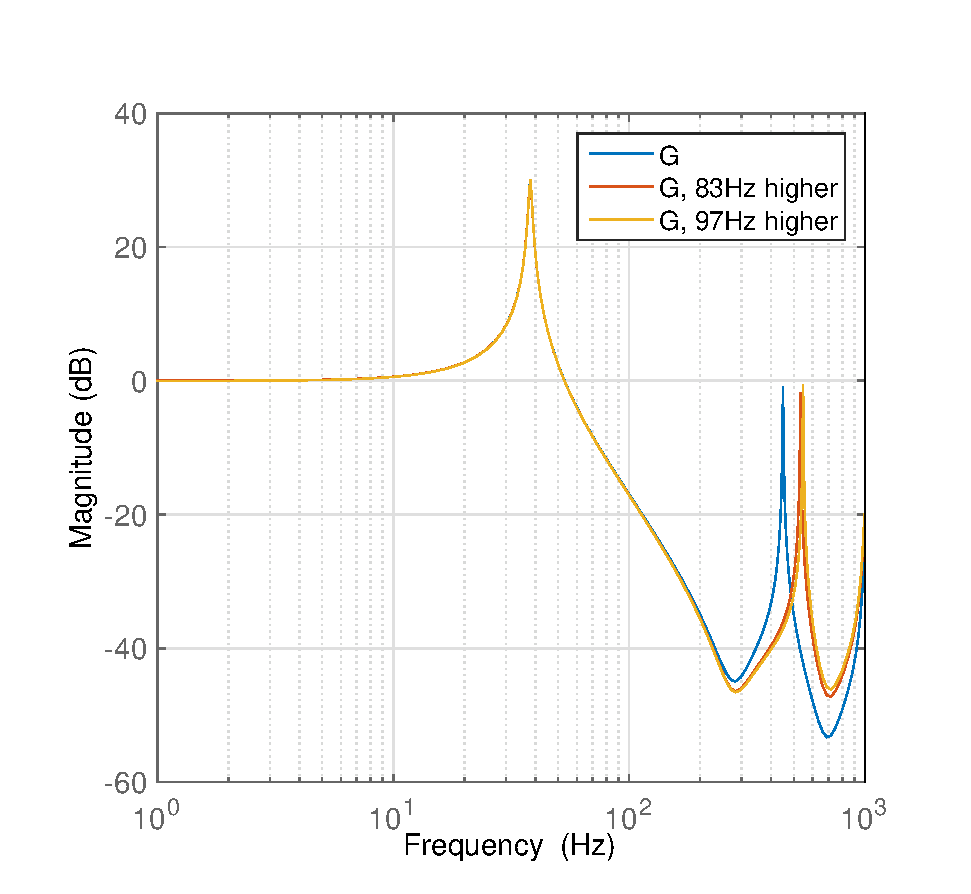
\includegraphics[width=0.65\textwidth]{fig/matlab/bode_high_model_error.eps}
  \caption{\label{fig:high_model_error} The \abbrFFT of the output signal for the \abbrIRC and the present approach, when applying a white noise to the output of G}
\end{figure}

\begin{figure}[h!]
  \centering %crop: left bottom right top
  \subfloat[][\label{fig:model_83}Model change of 83hz]{
  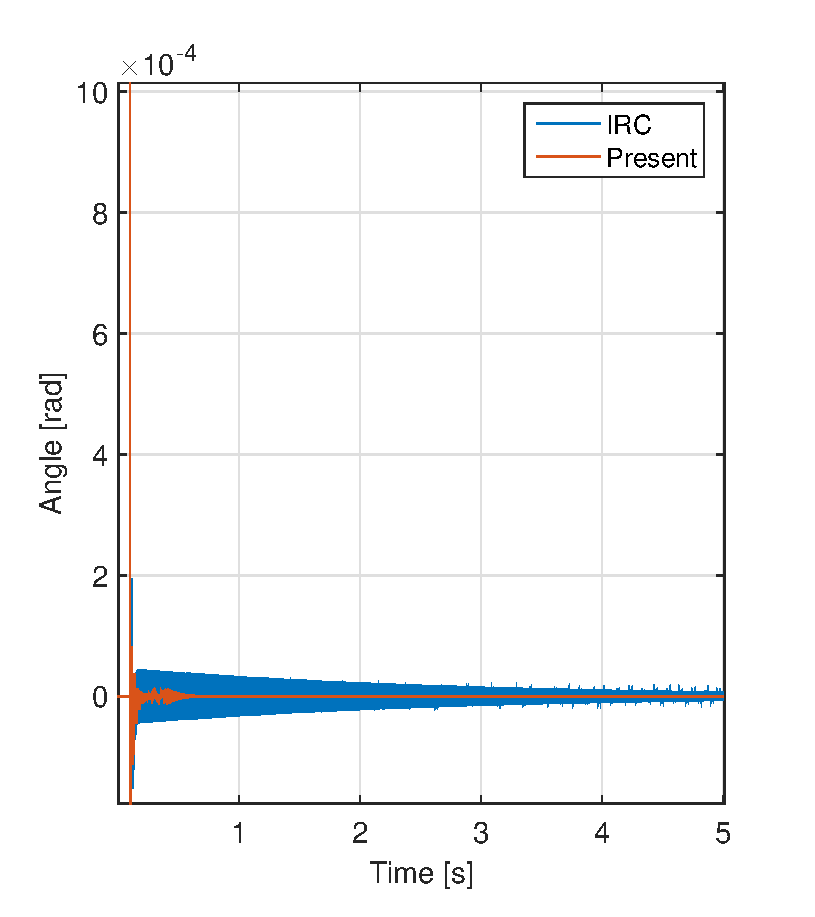
\includegraphics[width=0.46\textwidth, trim=0cm 0cm 1cm 0cm, clip=true]{fig/matlab/model_high_83hz.eps}}
  \qquad
  \subfloat[][\label{fig:model_97}Model change of 97hz]{
  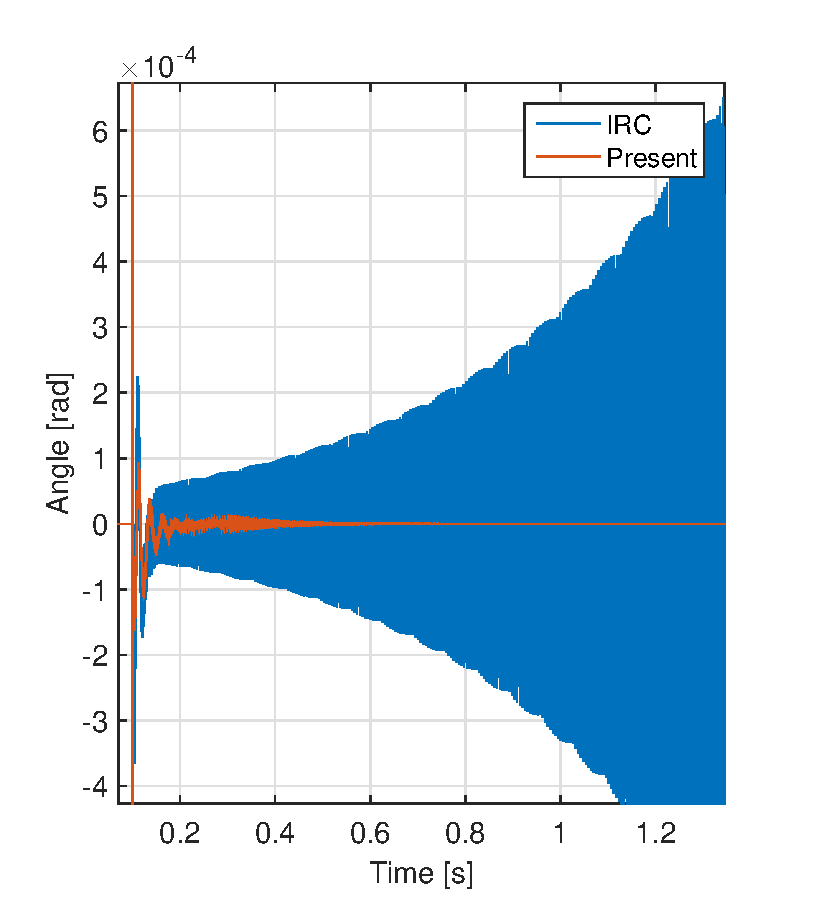
\includegraphics[width=0.46\textwidth, trim=0cm 0cm 1cm 0cm, clip=true]{fig/matlab/model_high_97hz.eps}}
  \caption{\label{fig:model_dist_high_order} Shows how the controller attenuates a disturbance impulse (amplitude of $5.1 \times 10^{-3}$) added to the output signal at $t=0.1s$. The highest resonance peak of G has in (a) been moved by 83Hz and in (b) by 97Hz.}
\end{figure}

\newpage
\FloatBarrier
\section{Harmonic Cancellation}
All harmonic cancellation methods were implemented and benchmarked with realistic disturbance data acquired with the lab setup described in \ref{sec:setup}. The disturbance data was acquired in open loop during a linear axis movement around the operating point on the linear axis, which is 3 mm out from the inner position with respect to the beam. Each cancellation method was benchmarked individually with respect to cancellation performance and robustness to model errors.

\subsection{Feedforward Disturbance Cancellation}\label{sec:hc}
The \abbrFDC methodology aims to cancel out known disturbances coming from a linear axis movement. The stepping signal sent to the motor is known at all time and is therefore suitable to be used as input signal ($d_0$ in Figure~\ref{fig:ffdist}) to the disturbance model. Data was acquired in open loop during a linear axis movement corresponding to 50 steps of the stepping motor. The movement was performed with four different speeds (1, 2, 5 and 10 steps/s) around the operating point. The chosen linear speeds were relatively low compared to normal operation, but used for the purpose of getting enough time between each step in order for the response to have sufficient time to settle. Figure~\ref{fig:stepinout} shows the yaw angle response from one motor step and the impulse used as input for the identification of the disturbance model. If this approach would be implemented on the real device, the stepping voltage would be used to form a pulse train containing impulses similar to the one showed in (a).

\begin{figure}[h!]
  \centering %crop: left bottom right top
  \subfloat[][Impulse used as input signal]{
  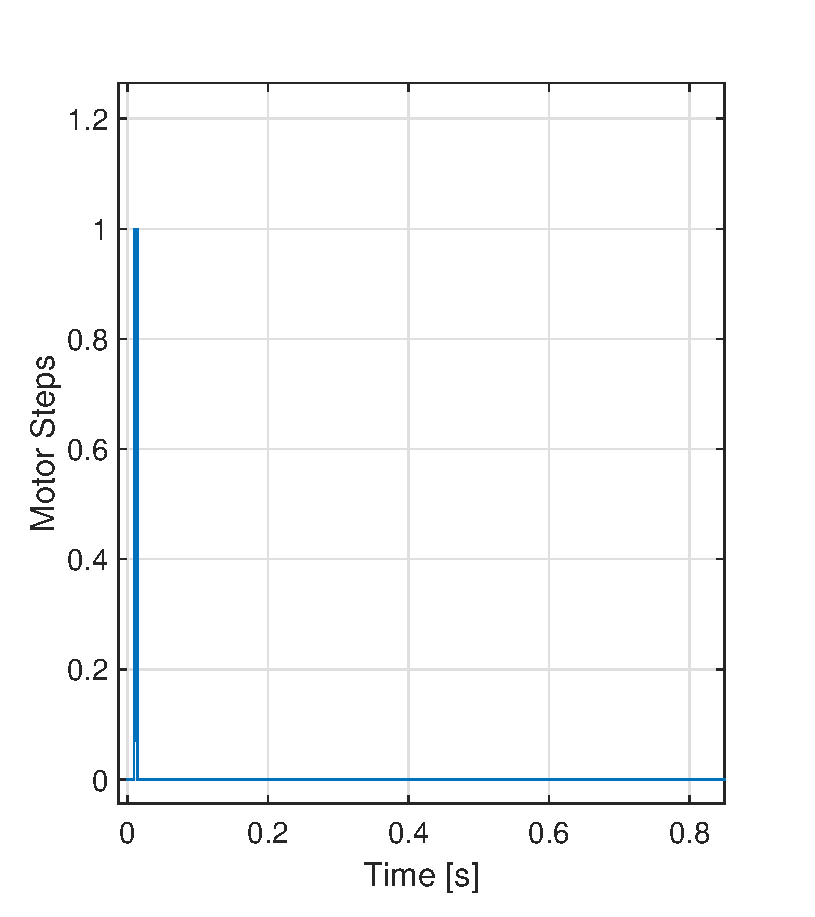
\includegraphics[width=0.46\textwidth, trim=0cm 0cm 1cm 0cm, clip=true]{fig/matlab/ff_impulse.eps}}
  \qquad
  \subfloat[][\label{fig:stepout}Mean of impulse responses]{
  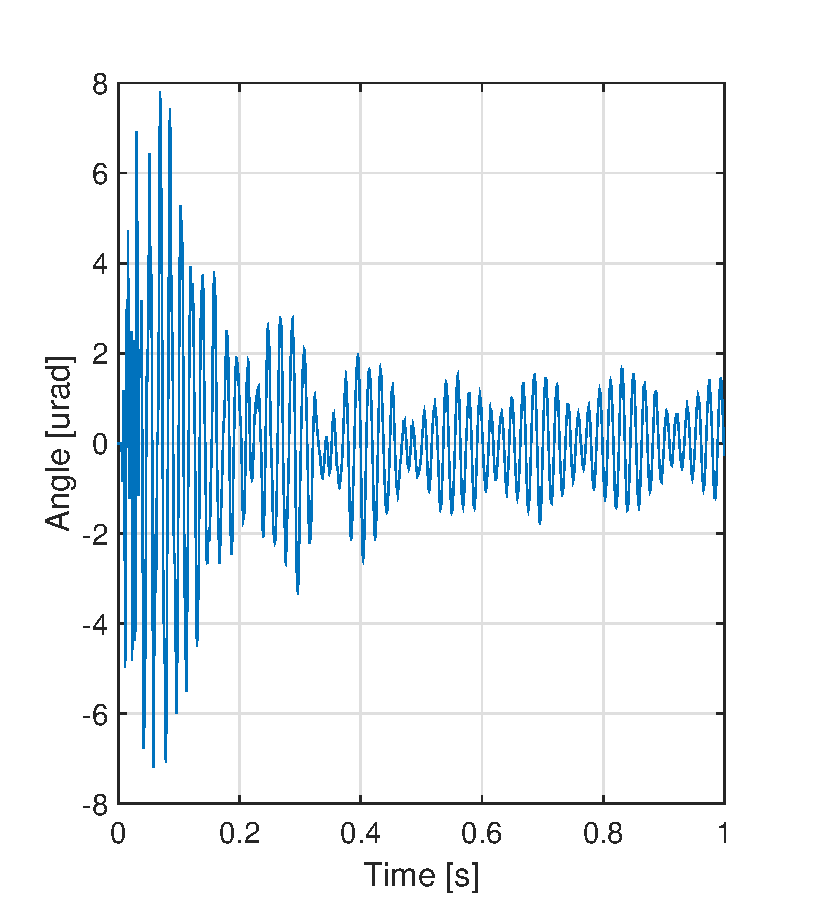
\includegraphics[ width=0.46\textwidth, trim=0cm 0cm 1cm 0cm, clip=true]{fig/matlab/yaw_angle_mean_1_step_s.eps}}
  \caption{\label{fig:stepinout} Shows the input signal (a) and the mean of 50 time-synchronized acquired step responses (b) at a movement of 1 step/s.}
\end{figure}

The empirical estimate of the disturbance model $P_d$ is obtained by dividing the \abbrFFT of (b) with the \abbrFFT of (a) in Figure~\ref{fig:stepinout}. The resulting empirical estimate is shown for different positions and speeds in Figure~\ref{fig:fft0_3} and \ref{fig:fft_6_5} .

\begin{figure}[h!]
  \centering %crop: left bottom right top
  \subfloat[][\abbrFFT at 0V ]{
  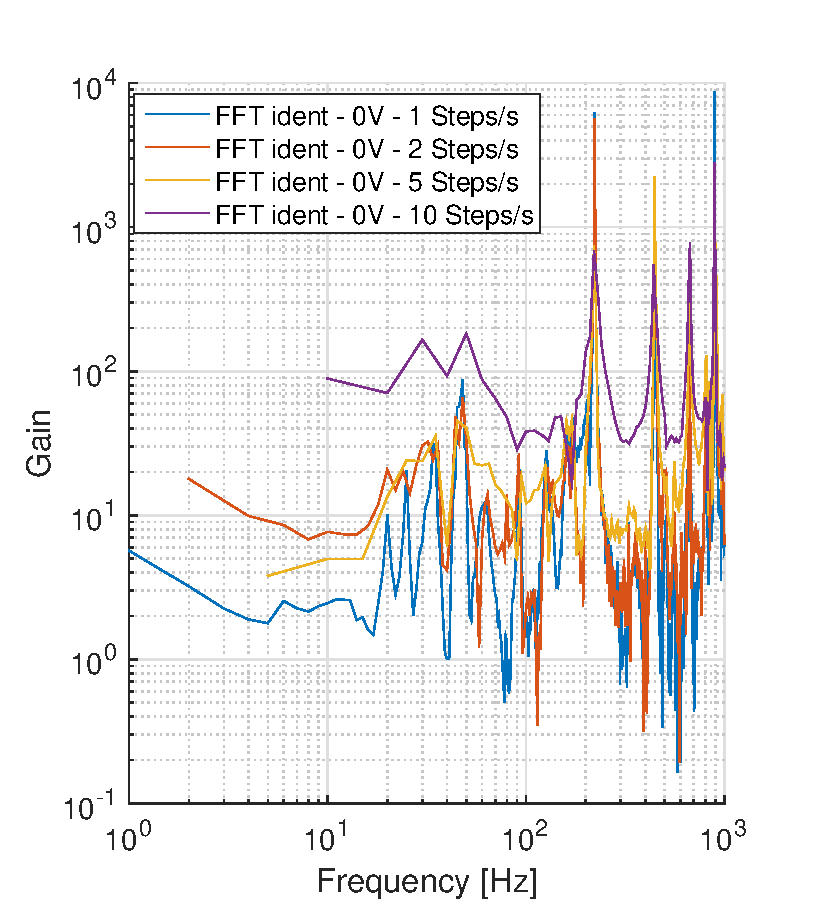
\includegraphics[width=0.46\textwidth, trim=0cm 0cm 0.9cm 0cm, clip=true]{fig/matlab/fft_mean_in_out_0V.eps}}
  \qquad
  \subfloat[][\abbrFFT at 3.25V]{
  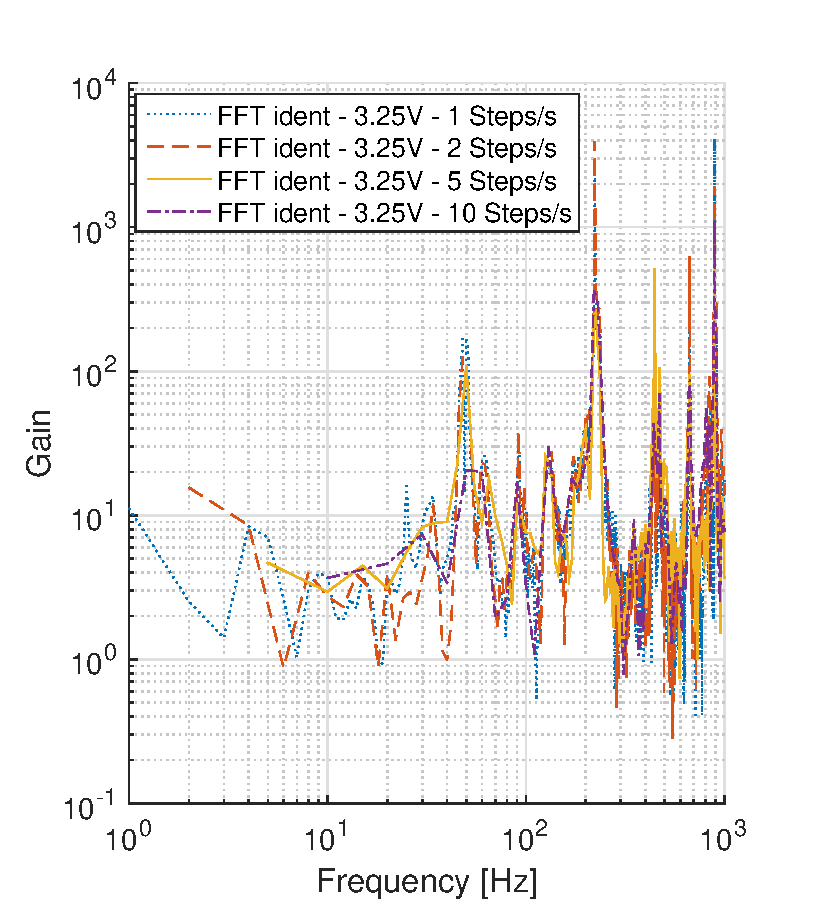
\includegraphics[width=0.46\textwidth, trim=0cm 0cm 0.9cm 0cm, clip=true]{fig/matlab/fft_mean_in_out_3V.eps}}
  \caption{\label{fig:fft0_3} \abbrFFT of the impulse response divided by the \abbrFFT of the impulse at two different positions, 0V: -10mrad (a) and 3.25: 0mrad (b) with different speeds.}
\end{figure}

\begin{figure}[h!]
  \centering %crop: left bottom right top
  \subfloat[][\label{fig:fft_6_5}\abbrFFT at 6.5V]{
  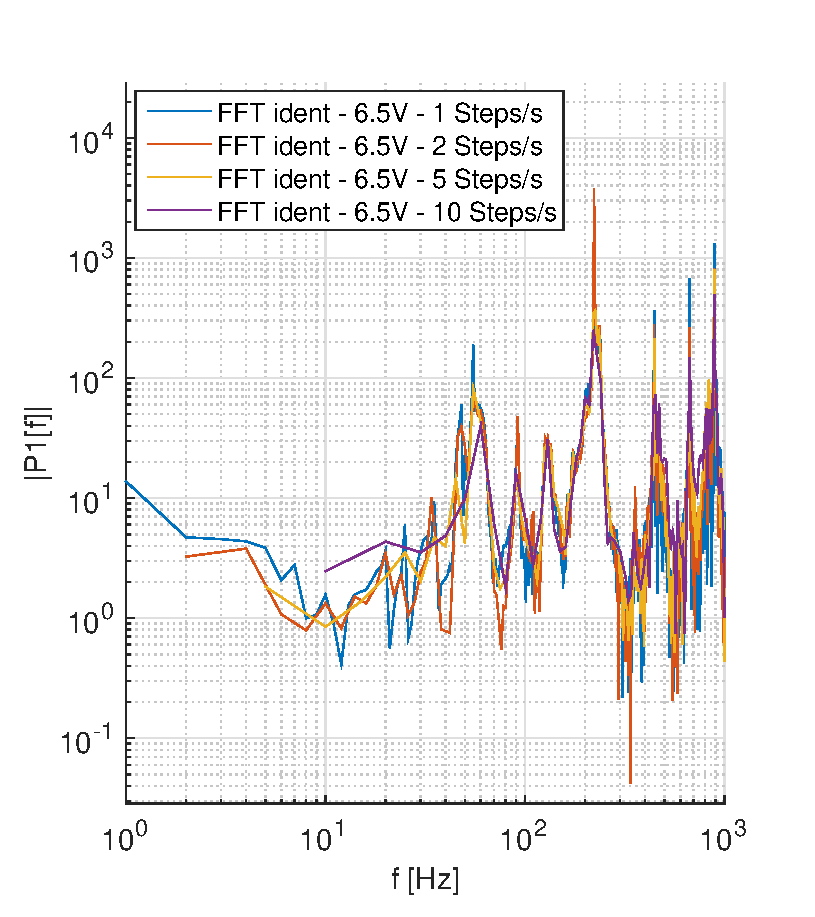
\includegraphics[width=0.46\textwidth, trim=0cm 0cm 1cm 0cm, clip=true]{fig/matlab/fft_mean_in_out_6_5V.eps}}
  \qquad
  \subfloat[][\label{fig:distmodelfit}Identified model]{
  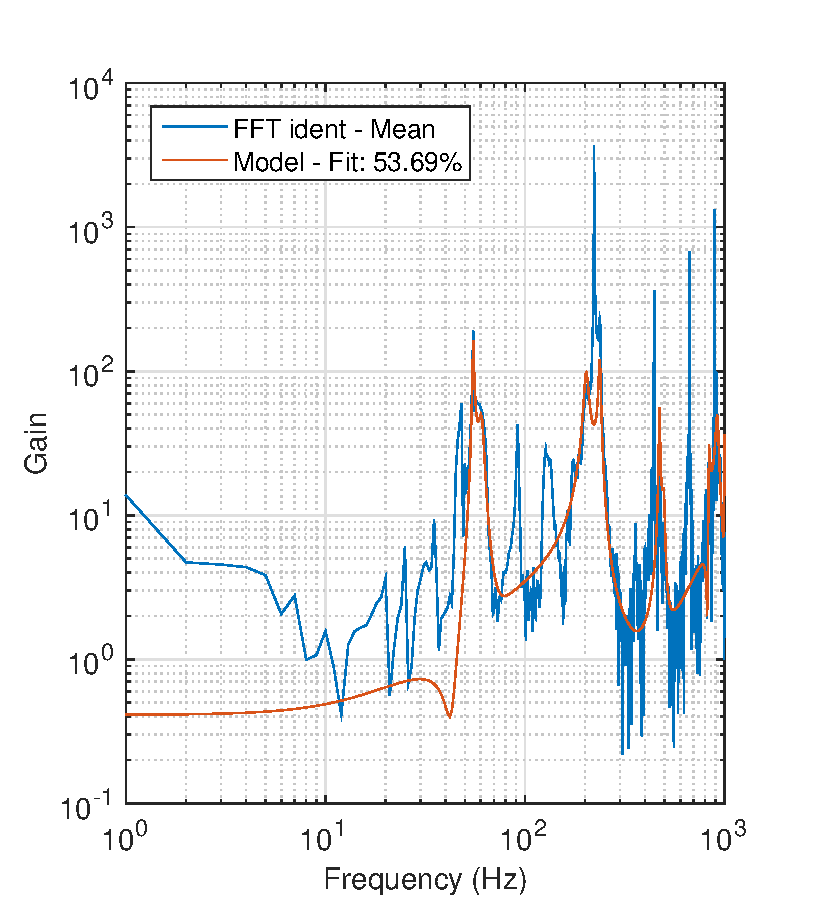
\includegraphics[width=0.46\textwidth, trim=0cm 0cm 1cm 0cm, clip=true]{fig/matlab/model_fit_1step_s.eps}}
  \caption{\label{fig:fft_6_5_modelfit} Shows the \abbrFFT of the impulse response divided by the \abbrFFT at 6.5V: 10mrad (a) at different speeds and the corresponding identified model (b).}
\end{figure}

As seen in the figures, the disturbance model have distinct peaks at around 220, 445, 670 and 890Hz. The resonance peak for a specific speed is a multiple of the stepping rate as seen in Figure~\ref{fig:3vzoomin}.

\begin{figure}[h!]
  \centering
  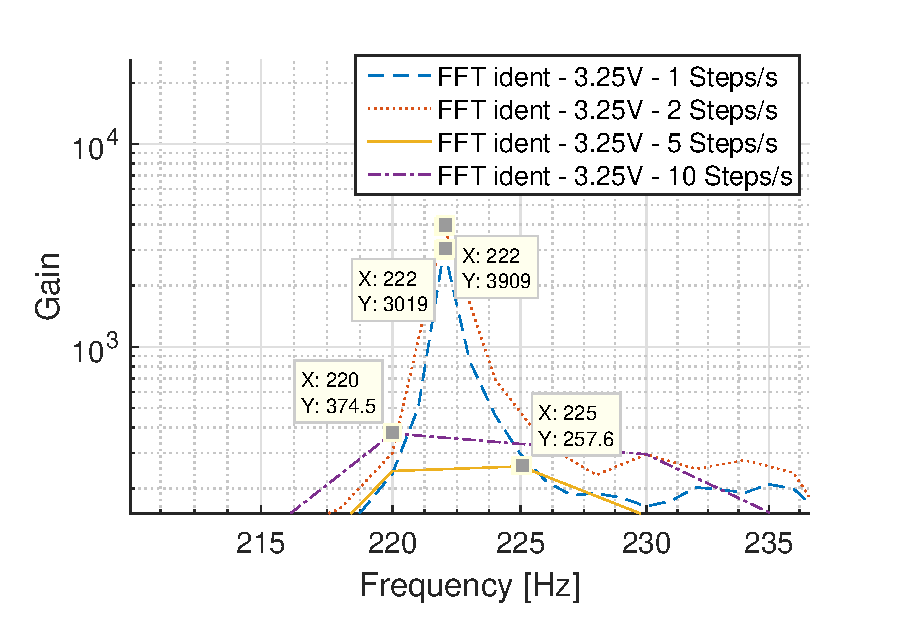
\includegraphics[width=0.7\textwidth]{fig/matlab/fft_mean_in_out_3V_zoomin.eps}
  \caption{\label{fig:3vzoomin} Zoom-in on the first resonance peak on the \abbrFFT performed on the data originating from the 3.25: 0mrad. The resonance peaks are clearly multiples of the stepping rate.}
\end{figure}
\FloatBarrier
Figure~\ref{fig:fft_6_5_modelfit} shows the identified model for the data acquired at 6.5V and 1 step/s. In order to sufficiently model four resonances, a 19 zeros and 20 poles transfer function was needed. The model is sufficient for simulations but has to be reduced for a reasonable implementation in terms of computational efficiency. The identification was performed using Matlab System Identification Toolbox with a selected frequency focus from 30-1000Hz. The identified disturbance model $P_d$ is presented in its final form in Appendix~\ref{app:fdc}. $K_f$ was calculated as $K_f=P_d/G$.
The disturbance model was benchmarked with 2 slightly different disturbances, first with the mean shown in Figure~\ref{fig:stepout} (the signal used in the identification) and then with a signal picked out as one period from the original acquired data. The cancellation performance  at 6.5V and 1 step/s can be seen in Figure~\ref{fig:benchmark_dist}. The \abbrFDC manages to mitigate the disturbance on the yaw angle by almost half of the amplitude with the mean fed as disturbance. With the more realistic disturbance in (b) the disturbance cancellation is however less effective.

\begin{figure}[h!]
  \centering %crop: left bottom right top
  \subfloat[][Mean as disturbance]{
  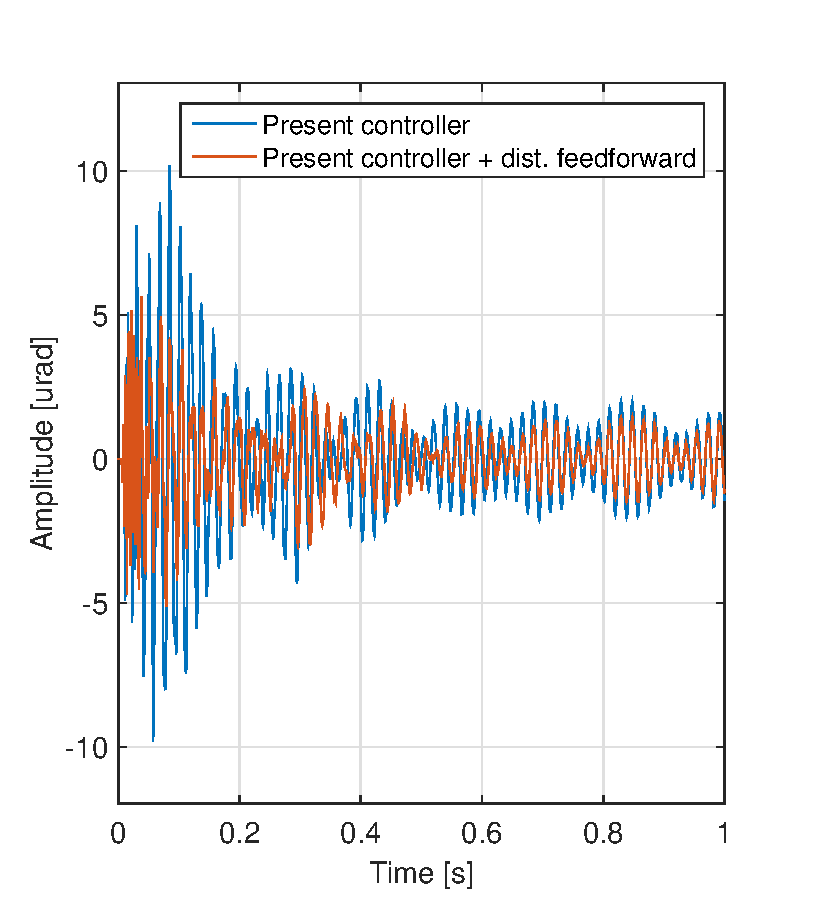
\includegraphics[width=0.46\textwidth, trim=0cm 0cm 1cm 0cm, clip=true]{fig/matlab/cancellation_1_step_s.eps}}
  \qquad
  \subfloat[][Original acquired signal as disturbance ]{
  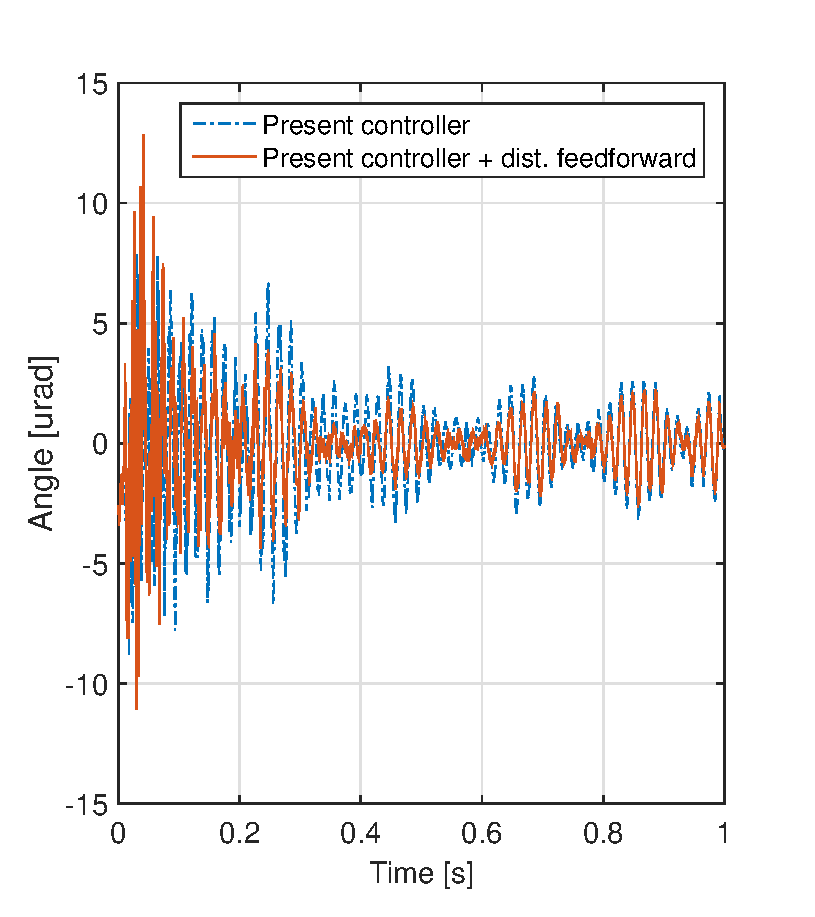
\includegraphics[width=0.46\textwidth, trim=0cm 0cm 1cm 0cm, clip=true]{fig/matlab/cancellation_1_step_s_real_dist.eps}}
  \caption{\label{fig:benchmark_dist} Shows the effect of the feedforward disturbance cancellation with the mean of the acquired response added as disturbance (a) and one period of the acquired response added as disturbance (b).}
\end{figure}
\FloatBarrier
To illustrate the model efficiency with different step rates, a benchmarking test with the same identified model as above was performed with the mean corresponding to each of the stepping rates added as disturbance. The outcome is presented in Table~\ref{tab:std_diff_speed} as the standard deviation of the yaw angle, showing that a single model is sufficient to reduce the disturbance level for several other stepping rates as well.
\begin{table}[h!]
  \centering
  \begin{tabular}{| l | l | l | l | l |}
    \hline
      Speed & 1 step/s & 2 step/s & 5 step/s & 10 step/s\\ \hline
      $\sigma_{Present}$ & 2.15 & 2.23 & 3.90 & 3.76\\
      $\sigma_{Present + dist.FF.}$ & 1.19 & 2.04 & 2.06 & 2.59\\
    \hline
  \end{tabular}
  \caption{\label{tab:std_diff_speed} Standard deviations of the output with and without disturbance feedforward for the different speeds with the mean of the acquired response corresponding to each speed added as disturbance. The model used in the disturbance feedforward was identified from the 6.5V and 1step/s data.}
\end{table}

\FloatBarrier
To benchmark how well the cancellation works with model errors, a simulation with four different perturbed models was performed with the disturbance feedforward based on the same models as before. The models including the original system itself is shown in Figure~\ref{fig:hc_me_bode}, where the first resonance peak has been perturbed. This models the previous identified behavior when the rotational stage rotates from -10 to 10mrad.

\begin{figure}[h!]
  \centering
  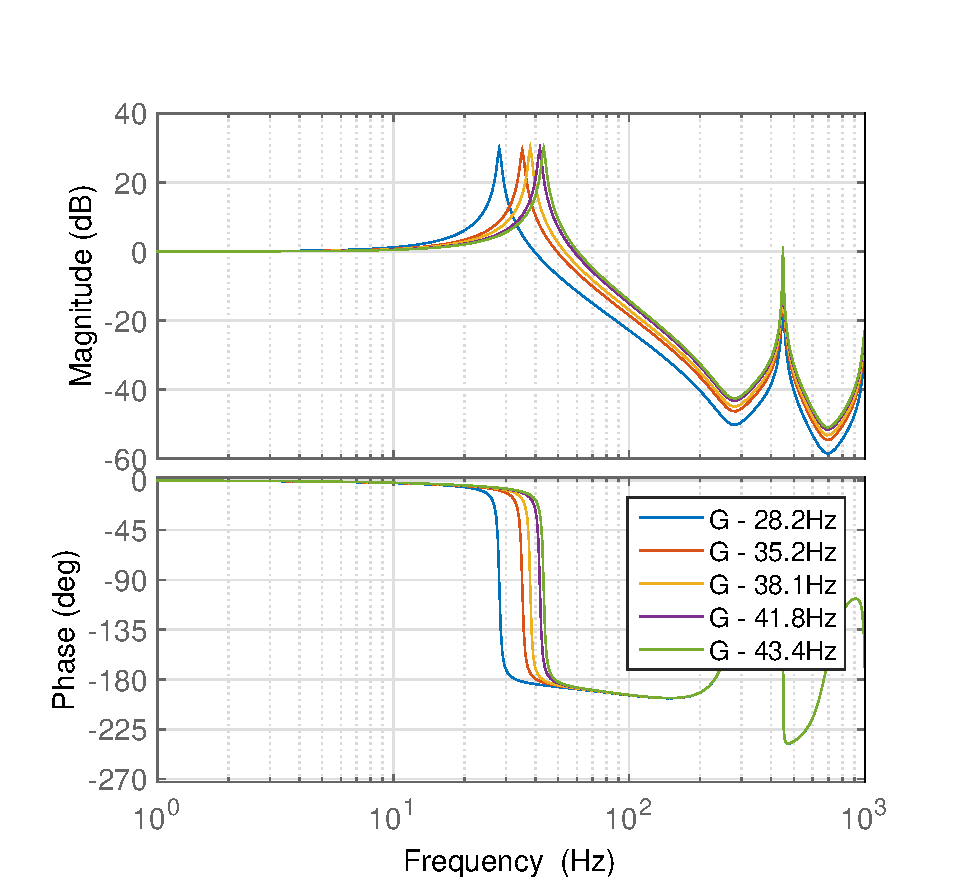
\includegraphics[width=0.7\textwidth]{fig/matlab/bode_rfdc_modelerror.eps}
  \caption{\label{fig:hc_me_bode} Bode diagram of the 5 different models used for the simulation of model error, including the original model G - 38.1Hz.}
\end{figure}

The \abbrFFT of the simulation results can be seen in Figure~\ref{fig:hc_model_error1} where the attenuation of the major disturbance component is shown. The simulations indicate that the cancellation is still efficient even with model errors being present. The original controller and system without disturbance cancellation is included in the plots as a reference and is named \emph{Present - 38.1 Hz}. Figure~\ref{fig:hc_model_error2} illustrates the impact that the model errors have to the attenuation of some other resonances present in the system. Here 92.3Hz is chosen as an example to illustrate that the cancellation with model errors can lead to amplification at some frequencies.


\begin{figure}[h!]
  \centering %crop: left bottom right top
  \subfloat[][\label{fig:hc_model_error1} Attenuation of major frequency]{
  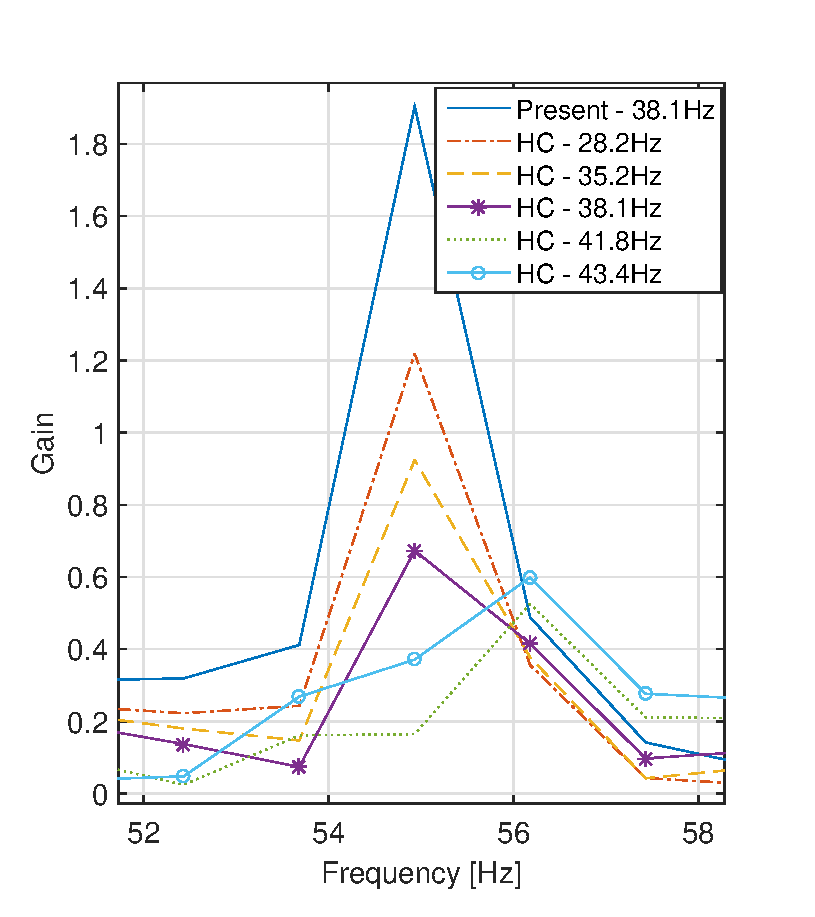
\includegraphics[width=0.46\textwidth, trim=0cm 0cm 1cm 0cm, clip=true]{fig/matlab/hc_model_error.eps}}
  \qquad
  \subfloat[][\label{fig:hc_model_error2} Impact on 92.3Hz component]{
  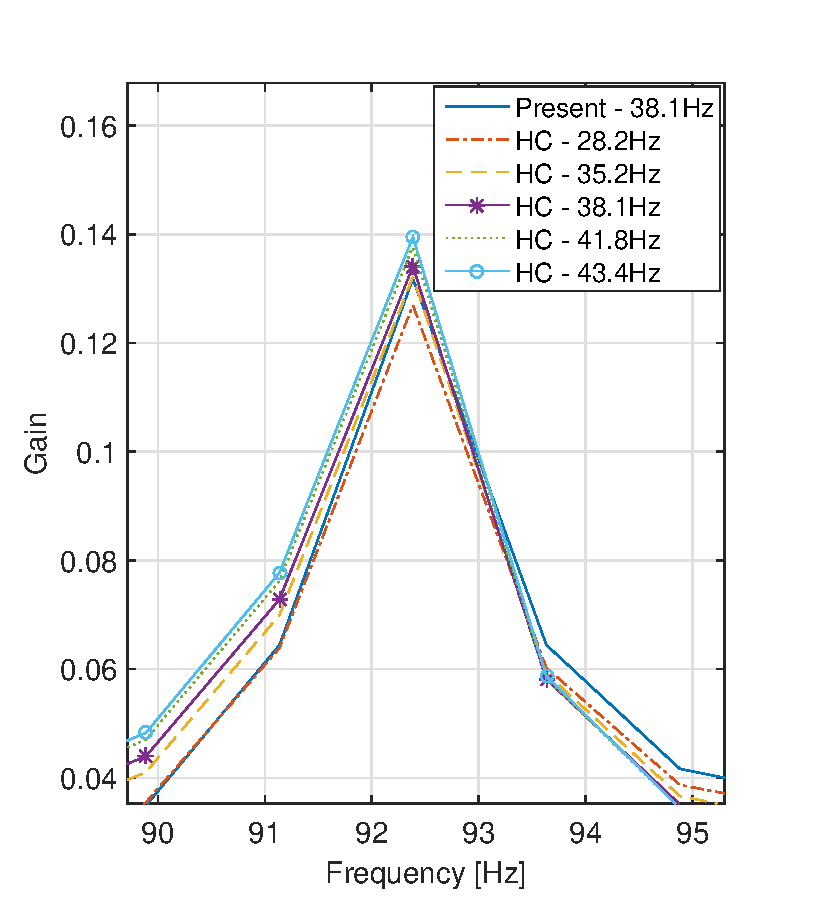
\includegraphics[width=0.46\textwidth, trim=0cm 0cm 1cm 0cm, clip=true]{fig/matlab/hc_model_error92.eps}}
  \caption{\label{fig:hc_model_error} Disturbance cancellation effectiveness with model errors. The attenuation of the major frequency is shown in (a) while the attenuation of the 92.3Hz component is shown in (b).}
\end{figure}


\FloatBarrier
\subsection{Cancellation with Internal Model Principle}
The implementation of the \abbrIMP cancellation method was based on the theory in Section~\ref{subsec:distimp}. A pure sinusoidal disturbance was used as the generating polynomial $\Gamma(s) = s^2 + \omega^2$, where the frequency to reject was chosen to $\omega = 2\pi50$. This choice of polynomial gives full attenuation in the selected frequency but impacts on the attenuation of system's first resonance peak at 38.1 Hz. Hence, in order to get sufficient attenuation at both of the frequencies, a bit of damping was added to the polynomial. The normalized continuous transfer function that was discretized and added to the system is presented below.

\begin{equation}
  C_{imp}(s) = \frac{(2pi50)^2}{s^2 + s + (2pi50)^2}
\end{equation}

The controller, shown in its full in \eqref{eq:imp_c}, was tuned using Matlabs's SISO-tool aiming to achieve equivalent performance as the present controller. The controller was based on a PI-controller with a notch filter to damp out higher order frequencies modes and a complex pair of zeros placed between the two resonance peaks at 38.1 and 50Hz to gain phase margin. Finally, a lead-filter was added to increase the phase margin even further.

\begin{equation}
  \label{eq:imp_c}
  C(z) = \frac{25.33z^7 - 130.6z^6 + 301.9z^5 - 429z^4 + 424.7z^3 - 291.5z^2 + 121.8z - 22.64}{z^7 - 3.6z^6 + 5.4z^5 - 4.5z^4 + 2.2z^3 - 0.63z^2 + 0.096z - 0.0061}
\end{equation}




Figure~\ref{fig:rfdc_s_gc} shows the resulting closed loop system and the sensitivity function from output disturbance to system output. The 2 drops in 38.1 and 50 Hz is clearly visible in the sensitivity function, but note that the attenuation of the 38.1 Hz is a bit less for the \abbrIMP approach. This phenomenon is sometimes called the \emph{waterbed effect} meaning that if the sensitivity to a disturbance is suppressed at one frequency it will increase in another.

\begin{figure}[h!]
  \centering %crop: left bottom right top
  \subfloat[][Closed loop system]{
  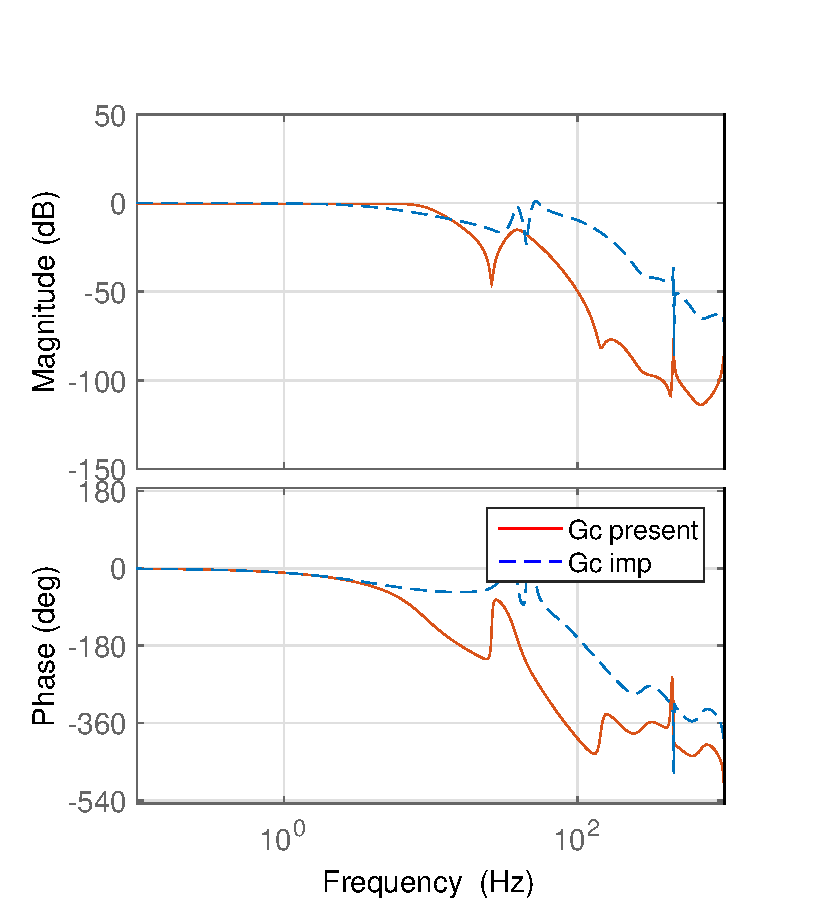
\includegraphics[width=0.46\textwidth, trim=0cm 0cm 1cm 0cm, clip=true]{fig/matlab/gc_imp.eps}}
  \qquad
  \subfloat[][Sensitivity function]{
  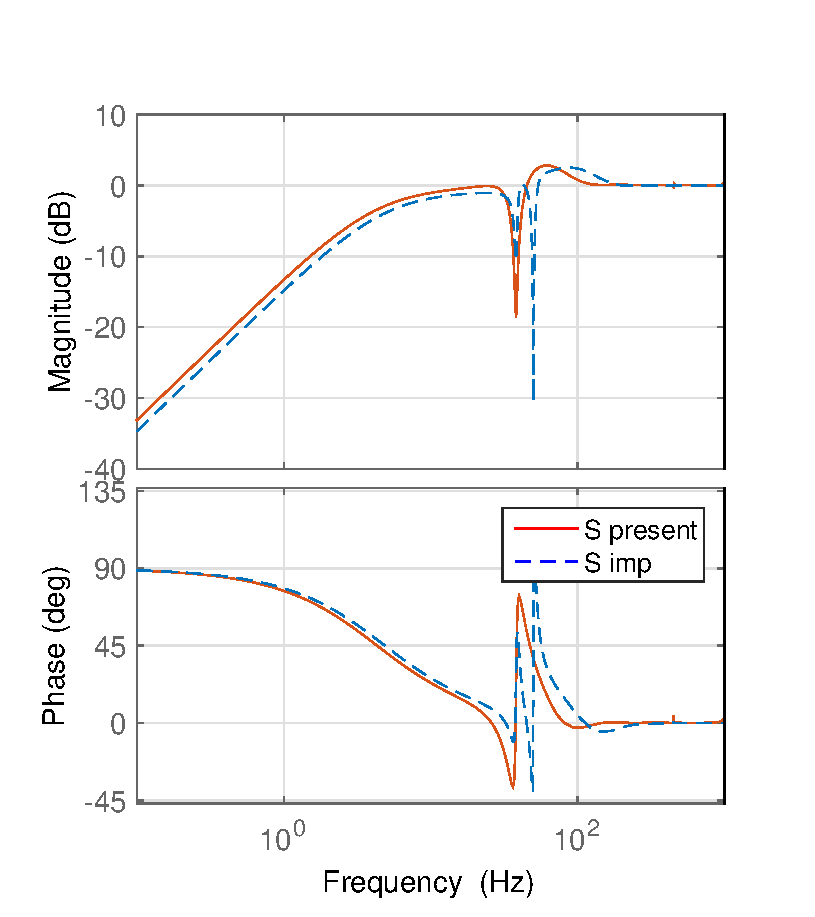
\includegraphics[width=0.46\textwidth, trim=0cm 0cm 1cm 0cm, clip=true]{fig/matlab/s_imp.eps}}
  \caption{\label{fig:rfdc_s_gc} Closed loop system (a) and sensitivity function, the transfer function from output disturbance to system output (b).}
\end{figure}

\FloatBarrier
The \abbrIMP method was benchmarked against the present controller in all tests. As a proof of concept, a 50Hz sinusoidal disturbance was added as a disturbance and the attenuation (in the perfect case) can be seen in Figure~\ref{fig:rfdc_p_atten}. The \abbrIMP managed to attenuate 96\% of the added disturbance. The missing 4 percent can be explained by the addition of damping that was added to the generating polynomial.

\begin{figure}[h!]
  \centering %crop: left bottom right top
  \subfloat[][Time domain]{
  \includegraphics[width=0.46\textwidth, trim=0cm 0cm 1cm 0cm, clip=true]{fig/matlab/distrej.eps}}
  \qquad
  \subfloat[][\abbrFFT]{
  \includegraphics[width=0.46\textwidth, trim=0cm 0cm 1cm 0cm, clip=true]{fig/matlab/distrej_fft.eps}}
  \caption{\label{fig:rfdc_p_atten} The time response is shown in (a) with cancellation of 50Hz component. The \abbrFFT performed on (a) after the response had settled is shown in (b).}
\end{figure}

For a more realistic benchmarking, disturbance data collected at 10 steps/s was added to the output of the system. The result is presented in Figure~\ref{fig:imp_realdata} where it is clear that the 50Hz component has been damped out efficiently.

\begin{figure}[h!]
  \centering
  \includegraphics[width=0.7\textwidth]{fig/matlab/distrej_realstep_fft.eps}
  \caption{\label{fig:imp_realdata} \abbrFFT performed on the output signal after the response had settled, with the acquired disturbance data as input signal.}
\end{figure}

\newpage~\newpage~
\FloatBarrier
Finally, the cancellation approach was tested for model robustness following the procedure described in Section~\ref{sec:hc}. The perturbed models used in the simulation can be seen in Figure~\ref{fig:hc_me_bode}. The attenuation of the selected frequency is presented in Figure~\ref{fig:imp_model_error1} showing that the cancellation is efficient for major model errors. One main drawback with this approach is depicted in Figure~\ref{fig:imp_model_error2} where the 130Hz component has been amplified due to the addition of the \abbrIMP cancellation strategy.


\begin{figure}[h!]
  \centering %crop: left bottom right top
  \subfloat[][\label{fig:imp_model_error1}Attenuation of selected frequency]{
  \includegraphics[width=0.46\textwidth, trim=0cm 0cm 1cm 0cm, clip=true]{fig/matlab/imp_model_error_real50.eps}}
  \qquad
  \subfloat[][\label{fig:imp_model_error2}Impact on 130Hz component]{
  \includegraphics[width=0.46\textwidth, trim=0cm 0cm 1cm 0cm, clip=true]{fig/matlab/imp_model_error_real.eps}}
  \caption{\label{fig:imp_model_error}  Disturbance cancellation effectiveness with model errors. The attenuation of the major frequency is shown in (a) with the unwanted attenuation of the 130Hz component is shown in (b).}
\end{figure}

\newpage
\FloatBarrier
\subsection{Repetitive Feedforward Disturbance Cancellation}
The Repetitive Feedforward Disturbance Cancellation (\abbrRFDC) method was implemented to reject three known disturbances. Hence, three second order disturbance models as given in \eqref{eq:sinm} were augmented as shown in \eqref{eq:augmentedres}. The chosen frequencies for cancellation were $w_1 = 2\pi60$, $w_2 = 2\pi90$ and $w_3 = 2\pi200$ rad/s.

\begin{subequations}
  \label{eq:augmentedres}
  \begin{alignat}{2}
    & \mathbf{A_{de}} = diag
    \begin{pmatrix}
      \begin{bmatrix}
         0 & 1\\[0.3em]
         -w_1^2 & 0
       \end{bmatrix}  &
       \begin{bmatrix}
          0 & 1\\[0.3em]
          -w_2^2 & 0
        \end{bmatrix} &
        \begin{bmatrix}
          0 & 1\\[0.3em]
          -w_3^2 & 0
        \end{bmatrix} \\
      \end{pmatrix} \\
    & \mathbf{C_{de}} =
        \begin{bmatrix}
            1 & 0 & 1 & 0 & 1 & 0 \\
        \end{bmatrix}
  \end{alignat}
\end{subequations}

These equations where augmented according to \eqref{eq:augumented} with the discrete time system matrices which can be seen in its full form in Appendix~\ref{app:rfdc}. The observer was implemented in state space form, with the following equations.

\begin{subequations}
\label{eq:augmented}
  \begin{alignat}{2}
    & \mathbf{A_{obs}} = \mathbf{A - KC} \\
    & \mathbf{B_{obs}} = \mathbf{[B, K]}^T \\
    & \mathbf{C_{obs}} = diag(\mathbf{C_{zs}, C_{zd}, C_{zd}, C_{zd}}) \\
    & \mathbf{D_{obs}} = zeros(4,2)
  \end{alignat}
\end{subequations}


A sufficient gain $K$ was calculated by using Kalman (\texttt{dlqe} in Matlab), with a high measurement (R) to process noise (Q) ratio, trusting in the predefined model. The values provided to the \texttt{dlqe} function are listed in \ref{tab:kalman}.

\begin{table}[h!]
  \centering
  \begin{tabular}{| l | l |}
    \hline
    Parameter & Value \\ \hline
    $R$ & $1$ \\
    $Q$ & $10^{-5}$ \\
    $G$ & $[1, 0, 0, 0, 0, 0, 10, 0, 8, 0, 70, 0]^T$ \\
    \hline
  \end{tabular}
  \caption{\label{tab:kalman} Parameters used for calculating the observer gain.}
\end{table}

The \abbrRFDC method was benchmarked against the present controller in all tests. As a proof of concept, three sinusoidal disturbances with frequencies $w_1$, $w_2$ and $w_3$ were added to the output of the system. Even though all of them were observed only $w_3$ was feedforwarded to cancel out the 200Hz component to begin with. The result is shown in Figure~\ref{fig:1_dist_both}, where it is clear that the 200Hz disturbance is perfectly canceled by the feedforward algorithm. Since 200Hz is a multiple of the sampling frequency $F_s = 2000Hz$, one period is sufficient to capture a full number of periods within the switching times. The switch was set to turn on (load one period) at $t_{on}=2s$ and to turn off at $t_{off}=2+1/200s$, which was the time when all the observed estimates had converged.

To prove the concept for multiple harmonic cancellation, all three of the estimated disturbances were added and subtracted from the input. To capture an even number of cycles, the switching times for the 60Hz an 90Hz were set to [$t_{on}=2s, t_{off}=2+6/60 s$] and [$t_{on}=2s, t_{off}=2+9/90 s$], respectively.

\begin{figure}[h!]
  \centering %crop: left bottom right top
  \subfloat[][\label{fig:1_dist} Time domain]{
  \includegraphics[width=0.46\textwidth, trim=0cm 0cm 1cm 0cm, clip=true]{fig/matlab/1_dist.eps}}
  \qquad
  \subfloat[][\label{fig:1_dist_fft} \abbrFFT]{
  \includegraphics[width=0.46\textwidth, trim=0cm 0cm 1cm 0cm, clip=true]{fig/matlab/1_dist_fft.eps}}
  \caption{\label{fig:1_dist_both} The time response is shown in (a) with cancellation of 200Hz after 2s. The \abbrFFT of (a) from t=2.5s to t=5s is shown in (b).}
\end{figure}

\begin{figure}[h!]
  \centering %crop: left bottom right top
  \subfloat[][\label{fig:3_dist} Time domain]{
  \includegraphics[width=0.46\textwidth, trim=0cm 0cm 1cm 0cm, clip=true]{fig/matlab/3_dist.eps}}
  \qquad
  \subfloat[][\label{fig:3_dist_fft} \abbrFFT]{
  \includegraphics[width=0.46\textwidth, trim=0cm 0cm 1cm 0cm, clip=true]{fig/matlab/3_dist_fft.eps}}
  \caption{\label{fig:3_dist_both} The time response is shown in (a) with cancellation of 60, 90 and 200Hz after 2s. The \abbrFFT of (a) from t=2.5s to t=5s is shown in (b).}
\end{figure}

The result is presented in Figure~\ref{fig:3_dist_both}, which also illustrates a perfect cancellation. Note that the \abbrFFT analysis is performed on data from t=2.5 to t=5s i.e. at the time when the feedforward cancellation has been added and the response has settled.

For a more realistic benchmarking, disturbance data collected at 10 steps/s was added to the output of the system. $w_1$, $w_2$ and $w_3$ are all major components of the acquired disturbance so the model in the observer were kept the same as before. The result presented in linear scale is shown in Figure~\ref{fig:fft_linear} where the modeled frequencies have been damped out efficiently. The gain of the 60Hz component for instance, is with the \abbrRFDC reduced to more than 1/8 of its original amplitude.

\begin{figure}[h!]
  \centering
  \includegraphics[width=0.7\textwidth]{fig/matlab/3real_dist_fft.eps}
  \caption{\label{fig:fft_linear} \abbrFFT of the added perturbation with and without cancellation of the 60Hz, 90Hz and the 200Hz component.}
\end{figure}

As seen in Figure~\ref{fig:fft_linear} the attenuation of the 200Hz is far from perfect. This is due to the higher noise level that now is present with the more realistic disturbance signal. A lower gain would reduce the noise in the observed disturbance, but would also lead to a longer converging time. Figure~\ref{fig:ph_lowgain} shows the \abbrFFT of the observed disturbance with a low gain and a settling time longer than 5 seconds. Figure~\ref{fig:ph_highgain} shows a less clean representation of the disturbance, achieved with a higher gain and a shorter settling time around 3 seconds.

\begin{figure}[h!]
  \centering %crop: left bottom right top
  \subfloat[][Time domain]{
  \includegraphics[width=0.46\textwidth, trim=0cm 0cm 1cm 0cm, clip=true]{fig/matlab/model_conv.eps}}
  \qquad
  \subfloat[][\abbrFFT]{
  \includegraphics[width=0.46\textwidth, trim=0cm 0cm 1cm 0cm, clip=true]{fig/matlab/model_conv_fft.eps}}
  \caption{\label{fig:ph_lowgain} Shows the convergence (a) of the 200Hz observed harmonic with $G = [1, 0, 0, 0, 0, 0, 10, 0, 8, 0, 10, 0]^T$. The \abbrFFT of (a) is shown in (b), showing a clean model of the 200 Hz component.}
\end{figure}

\begin{figure}[h!]
  \centering %crop: left bottom right top
  \subfloat[][Time domain]{
  \includegraphics[width=0.46\textwidth, trim=0cm 0cm 1cm 0cm, clip=true]{fig/matlab/model_conv_w.eps}}
  \qquad
  \subfloat[][\abbrFFT]{
  \includegraphics[width=0.46\textwidth, trim=0cm 0cm 1cm 0cm, clip=true]{fig/matlab/model_conv_fft_w.eps}}
  \caption{\label{fig:ph_highgain} Shows the convergence (a) of the 200Hz observed harmonic with $G = [1, 0, 0, 0, 0, 0, 10, 0, 8, 0, 70, 0]^T$. The \abbrFFT of (a) is shown in (b), including a lot of other frequency components in the 200 Hz harmonic model.}
\end{figure}

\FloatBarrier
An even higher gain would lead to a more noise added to the model and a reduction in cancellation performance which is illustrated in Figure~\ref{fig:convergence}, where it is clear that a shorter converge time implies in a reduction in cancellation performance. The figures show the cancellation of the 200Hz component with a converge time of 2s in (a) achieved with a gain of 70 as before and a converge time of 1s in (b) achieved with a gain of 140.

\begin{figure}[h!]
  \centering %crop: left bottom right top
  \subfloat[][Converged within 2s]{
  \includegraphics[width=0.46\textwidth, trim=0cm 0cm 1cm 0cm, clip=true]{fig/matlab/converge70.eps}}
  \qquad
  \subfloat[][Converged within 1s]{
  \includegraphics[width=0.46\textwidth, trim=0cm 0cm 1cm 0cm, clip=true]{fig/matlab/converge140.eps}}
  \caption{\label{fig:convergence} Shows the cancellation performance for 200Hz with a model state convergence of 2s in (a) and 1s in (b).}
\end{figure}

To overcome this issue, a bandpass filter could be added to reduce the noise level of the model and thereby enabling for quicker convergence. The bandpass filter stated in \eqref{eq:bandpass} was used in the simulations with $\omega=2\pi 200$, $k=1/100$, $\xi_a=1$ and $\xi_b=0.01$, which has zero phase shift for signals entering at 200Hz, but shifts all other frequencies. Tests where performed with this filter but without any increase in disturbance cancellation performance.

To benchmark the sensitivity to model errors, a similar simulation as in Section~\ref{sec:hc} was performed on the \abbrRFDC method. The perturbed models used in the simulation can be seen in Figure~\ref{fig:hc_me_bode}. The attenuation of the selected frequency is shown in Figure~\ref{fig:rfdc_model_error1} showing that the cancellation is efficient with low model errors, but amplifies the component if the error is too large (\abbrRFDC - 43.4 Hz in figure). Figure~\ref{fig:rfdc_model_error2} illustrates that the \abbrRFDC is not amplifying other major frequencies components by showing one example e.g. the 130 Hz component.

\begin{figure}[h!]
  \centering %crop: left bottom right top
  \subfloat[][\label{fig:rfdc_model_error1} Attenuation of selected frequency]{
  \includegraphics[width=0.46\textwidth, trim=0cm 0cm 1cm 0cm, clip=true]{fig/matlab/rfdc_model_error_real60.eps}}
  \qquad
  \subfloat[][\label{fig:rfdc_model_error2} Impact on 130Hz component]{
  \includegraphics[width=0.46\textwidth, trim=0cm 0cm 1cm 0cm, clip=true]{fig/matlab/rfdc_model_error_real.eps}}
  \caption{\label{fig:rfdc_model_error} Disturbance cancellation effectiveness with model errors. The attenuation of the major frequency is shown in (a) while the attenuation of the 130Hz component is shown in (b).}
\end{figure}

\newpage
\FloatBarrier
\section{Comparison}\label{sec:comparison}
This section compares and summarizes the stand-alone control approaches (\abbrIRC and \abbrMRACPE) and the approaches that aims to cancel harmonics (\abbrFDC, \abbrRFDC and \abbrIMP). Table~\ref{tab:comp_h} and \ref{tab:comp} summarizes comparable results presented in previous sections. Key values from the graphs have been collected to give the reader an overview of the achieved performance for each control approach.

In Table~\ref{tab:comp}, the closed-loop bandwidth is presented for each approach, where "-" means that a theoretical bandwidth is missing for the \abbrMRACPE. The tracking error (nr 3-7) is presented as the standard deviation of the difference between reference and output signal, acquired after each approach has settled. The tracking error with model errors being present is shown in nr 4-7. Here, infinite tracking error means that the system is unstable. First resonance peak frequencies are selected to put the system on the border of instability. Nr 7 presents the disturbance rejection with a disturbance added to the system output, measured in settling time from the time when the disturbance was added.

\begin{table}[h!]
  \centering
  \begin{tabular}{| l | P{3.4cm} | P{2.2cm} | P{2.2cm} | P{2.8cm} |}
    \hline
    \bf{Nr} & \bf{Aspect}  & \bf{Present} & \bf{\abbrIRC} & \bf{\abbrMRACPE} \\ \hline
    1 & Closed-loop Bandwidth [Hz] & 9.7 & 73.3 & -\\ \hline
    2 & Gain/Phase margin [dB / $^{\circ}$] & 14.4/66.2 & 13.1/49.4 & -\\ \hline
    3 & Tracking error, periodic input $\sigma$-[mrads] & $0.29$ & $0.03$ & $0.11$\\ \hline
    4 & Tracking error with model errors (model's 1st resonance at 22.0Hz), $\sigma$-[mrads] & $\infty$ & 0.03 & 0.21\\ \hline
    5 & Tracking error with model errors (model's 1st resonance at 67.2Hz), $\sigma$-[mrads] & $\infty$ & 0.03 & 0.11\\ \hline
    6 & Tracking error with model errors (model's 1st resonance at 17.6Hz), $\sigma$-[mrads] & $\infty$ & $\infty$ & 0.47\\ \hline
    7 & Tracking error with model errors (model's 1st resonance at 77.7Hz), $\sigma$-[mrads] & $\infty$ & $\infty$ & 0.11\\ \hline
    8 & Output disturbance rejection, settling time (1\%) [ms] & 8 & 25 & 260\\ \hline
    9 & Input/Output disturbance rejection, $\sigma$-[\unit{\micro\radian}] & $0.68 $/$1.43$ & $0.45$/$1.46$ & $1.95$/$1.41$\\ \hline
    10 & Stability issues & Unstable with high model errors & Unstable with high model errors, but better than present & Good adaption even with model errors, but tuning for quicker adaption easily leads to instability.  Stability only proven in continuous time. \\ \hline
    11 & Design and implementation considerations & Straight- forward technique, allowing for basic stability analysis & Same as present & Hard to tune. High computational burden for higher order models.\\ \hline
  \end{tabular}
  \caption{\label{tab:comp} Key parameters for all stand-alone control approaches.}
\end{table}

\FloatBarrier
In Table~\ref{tab:comp_h}, the cancellation effectiveness is measured as attenuation of the resonance peak with respect to the present approach. For aspect nr 3 and 4, the attenuation is measured with respect to the present controller that also includes the perturbed model written in the parentheses. 

\begin{table}[h!]
  \centering
  \begin{tabular}{| l | P{3.7cm} | P{2.2cm} | P{2.2cm} | P{2.2cm} |}
    \hline
      \bf{Nr} & \bf{Aspect} & \bf{\abbrFDC} & \bf{\abbrRFDC} & \bf{\abbrIMP} \\ \hline
    1 & Affecting closed loop system & No & No & Yes\\ \hline
    2 & Cancellation effectiveness of major frequency, attenuation-[\%]                & 64.6 & 88.4 & 83.3\\ \hline
    3 & Cancellation with model errors (model's 1st resonance at 28.2Hz), attenuation-[\%] & 40.5 & 26.6 & 73.5\\ \hline
    4 & Cancellation with model errors (model's 1st resonance at 43.4Hz), attenuation-[\%] & 57.7 & 5.0 & 83.4\\ \hline
    5 & Implementation considerations & Requires high order model, computational demanding. & Requires observer, computational demanding. Can be used as add-on.& Controller must be retuned 6 when selecting another frequency. \\ \hline
  \end{tabular}
  \caption{\label{tab:comp_h} Key parameters for all harmonic cancellation control approaches.}
\end{table}
